\documentclass[11pt, a4paper]{report}

% --- PACKAGES ---
\usepackage[a4paper, margin=2.5cm]{geometry}
\usepackage{microtype}
\usepackage{graphicx}
\usepackage{titlesec}
\usepackage{tocloft}
\usepackage{booktabs}
\usepackage{enumitem}
\usepackage{listings}
\usepackage{fancyhdr}
\usepackage{amsmath}
\usepackage[table]{xcolor}
\usepackage[backend=biber,style=numeric,sorting=none]{biblatex}
\addbibresource{references.bib}

% FONTS (LuaLaTeX): New Computer Modern for serif, sans and math (loads
% fontspec + unicode-math); JetBrains Mono for code
\usepackage{newcomputermodern}

% Emoji fallback (LuaLaTeX + luaotfload). The Nerd Font covers U+26A0 but not
% the other emoji in the listed source (U+274C, U+1F449, U+1F4BE, ...).
\directlua{
  luaotfload.add_fallback("monofontemoji", {
      "Apple Color Emoji:mode=harf;"
  })
}

\setmonofont{JetBrainsMono Nerd Font Mono}[Scale=MatchLowercase,RawFeature={fallback=monofontemoji}]

% --- HYPERLINKS STYLING ---
\usepackage[pdfusetitle]{hyperref}
\usepackage{xurl} % allow long URLs to break across lines
\hypersetup{
  colorlinks=false,
  linkcolor=blue,
  citecolor=blue,
  urlcolor=cyan,
}
\urlstyle{same}

% --- TABLE STYLING ---
\definecolor{TableHeader}{RGB}{30, 34, 40}  % Dark slate
\definecolor{TableRow}{RGB}{245, 245, 245}   % Light gray

\setlist[itemize]{label=--}
\setlength{\parskip}{0.5em}
\setlength{\parindent}{0pt}

% Fix fancyhdr warning about headheight
\setlength{\headheight}{14pt} % or 15pt

% --- CODE STYLING ---
\definecolor{codegreen}{rgb}{0,0.6,0}
\definecolor{codegray}{rgb}{0.5,0.5,0.5}
\definecolor{codepurple}{rgb}{0.58,0,0.82}
\definecolor{backcolour}{rgb}{0.95,0.95,0.92}

\lstdefinestyle{pythonstyle}{
  backgroundcolor=\color{backcolour},
  commentstyle=\color{codegreen},
  keywordstyle=\color{magenta},
  numberstyle=\tiny\color{codegray},
  stringstyle=\color{codepurple},
  basicstyle=\ttfamily\footnotesize,
  breakatwhitespace=false,
  breaklines=true,
  captionpos=b,
  keepspaces=true,
  numbers=left,
  numbersep=5pt,
  showspaces=false,
  showstringspaces=false,
  showtabs=false,
  tabsize=2,
  language=Python
}
\lstset{style=pythonstyle}
% Ignore emoji variation selectors (U+FE0F) in listed source; the harf emoji
% fallback crashes on them.
\catcode"FE0F=9

% --- HEADER/FOOTER ---
\pagestyle{fancy}
\fancyhf{}
\rhead{\textbf{Technical Report}}
\lhead{Jackson Ferguson}
\cfoot{\thepage}

% --- TITLE FORMATTING ---
\titleformat{\chapter}[display]
{\normalfont\huge\bfseries}{\chaptertitlename\ \thechapter}{20pt}{\Huge}

% =============================================================================
% DOCUMENT START
% =============================================================================
\begin{document}

% --- TITLE PAGE ---
\begin{titlepage}
  \centering
  \vspace*{2cm}

  {\Huge \textbf{From Python to Silicon}}

  \vspace{0.5cm}
  {\Large A Technical Report on \\ Logistics, Power, Analog Synthesis, and Signal Analysis}

  \vspace{1.5cm}

  \textbf{Jackson Ferguson}\\
  \textit{University of Victoria}\\
  \textit{Astrophysics}

  \vspace{2cm}

  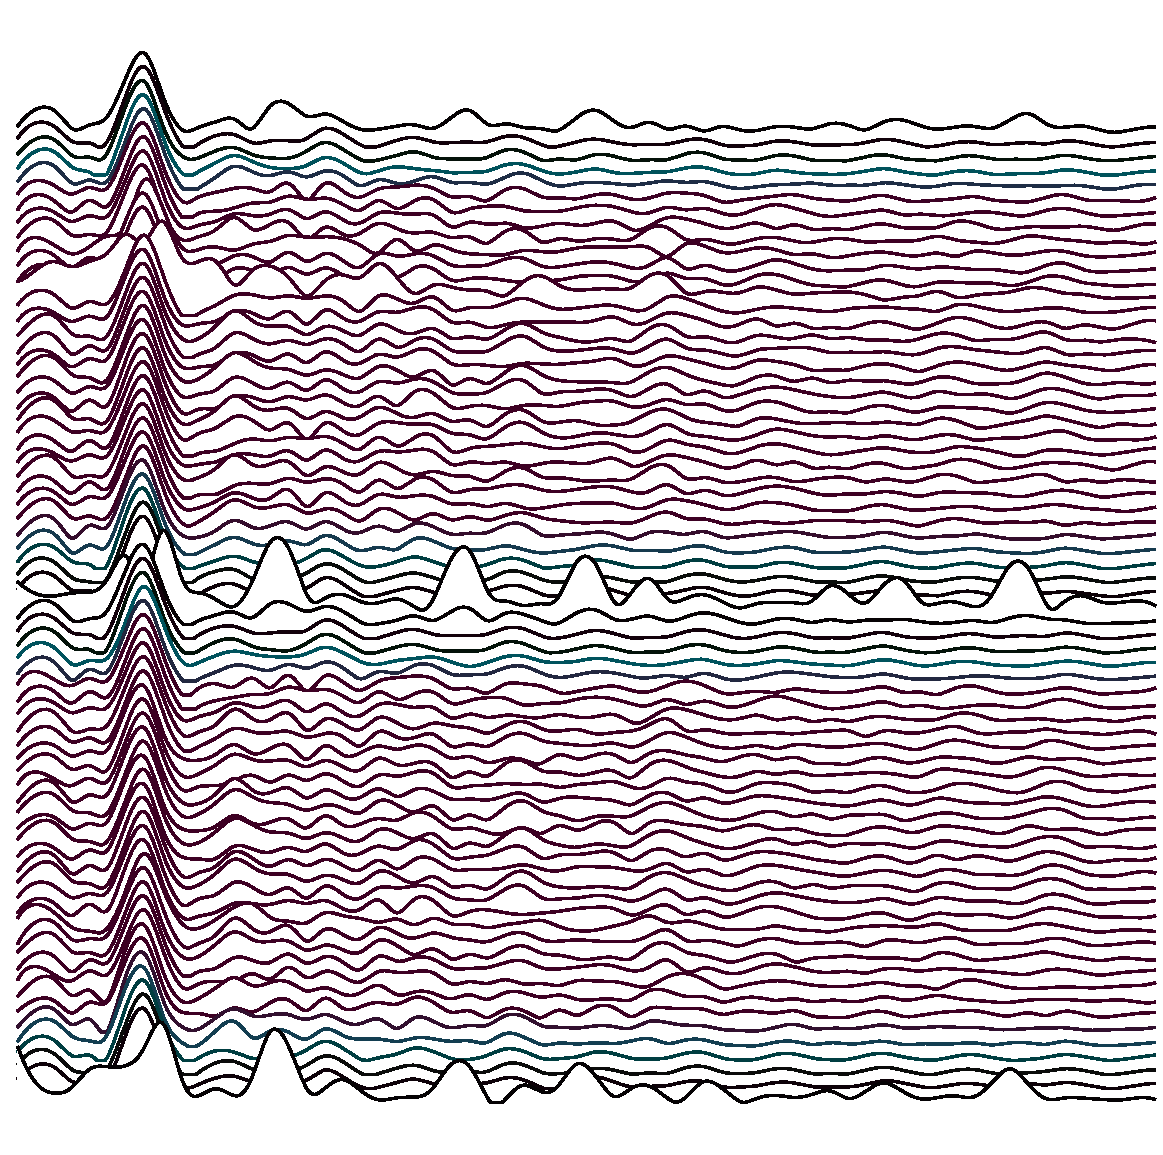
\includegraphics[width=0.5\pagewidth]{figures/harmonic_landscape.pdf}

  {\scriptsize\textit{Title graphic generated by the author (Python); source code in the accompanying repository:
  \url{https://github.com/JacksonFergusonDev/systems-audio-lab}.}}

  \vfill

  {\large \today}

\end{titlepage}

% --- ABSTRACT ---
\begin{abstract}
  \noindent This report documents building the tools needed to build, and then measure, one device: an analog guitar pedal (the Red Llama). My background is in software, and the usual hobbyist workflow gave me no way to check parts orders, supply noise or the pedal's actual behavior, so I built those tools as well.

  The report covers four systems, each supporting the next: (1) \href{https://github.com/JacksonFergusonDev/star-ground}{\textbf{Star Ground}}, a rule-based Python tool that turns bills of materials (BOMs) into parts orders; (2) a heatsinked \textbf{linear power supply}; (3) the \textbf{Red Llama} analog overdrive circuit; and (4) an \textbf{RP2040 data acquisition system} (DAQ), used to measure the pedal's harmonic distortion and its swept frequency response.
\end{abstract}

\tableofcontents
\newpage

% =============================================================================
% INTRODUCTION
% =============================================================================
\chapter{Introduction}

\section{Motivation}
Computational astrophysics models complex systems precisely, but the systems stay virtual. As an undergraduate working mostly on data pipelines in Python, I work in environments where the same input always gives the same output. Moving from software to physical hardware breaks that assumption; I refer to this as the ``Full-Stack Gap.''

Physical systems have sources of variation that code does not: component tolerances, thermal drift, unreliable supply chains and electromagnetic interference. The immediate goal of this project was to build one analog device (the Red Llama Overdrive). The broader goal was to apply software engineering practices (modularity, regression testing and version control) to building hardware.

\section{Problem Formulation}
The usual hobbyist workflow relies on ad-hoc solutions and judging results by ear. It has three weaknesses that make results hard to reproduce or measure:

\begin{enumerate}
  \item \textbf{Logistics:} A package manager resolves software dependencies in seconds; hardware dependencies have to be ordered and shipped. Managing a bill of materials (BOM) by hand is error-prone, and one missing resistor can stall a project for weeks.

  \item \textbf{Power:} High-gain audio stages are sensitive to power supply noise, and consumer switch-mode power supplies (SMPS) produce high-frequency switching ripple \cite{ti_an1950_lownoise_smps}. A generic adapter adds an uncontrolled noise source to the signal path.

  \item \textbf{Validation:} Audio circuits are usually judged by ear (``it sounds good''). But tone can be measured, as harmonic distortion and frequency response. Without a calibrated instrument, design changes are trial and error.
\end{enumerate}

\section{Approach}
To address these, I built the tools needed to build and measure the device rather than buying them. Every stage of the signal chain, from ordering the parts to analyzing the output, is then documented and under my control.

This report covers the design, construction and integration of four systems:

\begin{itemize}
  \item \textbf{\href{https://github.com/JacksonFergusonDev/star-ground}{Star Ground} (Logistics):} A Python tool that treats hardware BOMs as structured data. It parses PDF build documents into JSON and computes the order from them, removing manual transcription from the ordering process.

  \item \textbf{Linear Power Regulator (Infrastructure):} A heatsinked 12V-to-9V linear supply based on the L7809. It is intended to keep the wall adapter's switching ripple out of the device under test (DUT), so that what appears in the output comes from the device. Its output ripple has not been measured.

  \item \textbf{Red Llama Overdrive (Device Under Test):} The device being measured. This analog circuit biases a CD4049 CMOS hex inverter, a digital logic chip, into its linear region and uses it as an amplifier. The hypothesis is that it saturates softly, like a vacuum tube triode.

  \item \textbf{RP2040 DAQ (Instrumentation):} An FFT spectrum analyzer built from an RP2040 microcontroller and an analog front end (AFE). Its sample rate is calibrated against crystal-referenced test tones, so the DUT's harmonic content can be measured rather than judged by ear.
\end{itemize}

\section{Report Structure}
The chapters follow the order in which the systems were built:
\begin{itemize}
  \item \textbf{Chapter 2} describes Star Ground, the parts-ordering software.
  \item \textbf{Chapter 3} describes the power supply.
  \item \textbf{Chapter 4} describes the analog circuit and how it was built.
  \item \textbf{Chapter 5} describes the measurement instrument and its calibration.
  \item \textbf{Chapter 6} presents the measurements and tests the hypotheses above.
\end{itemize}

Every measured value in Chapters 5 and 6 is computed in the Jupyter notebooks in \texttt{oscilloscope-rp2040/notebooks/} of the accompanying repository (\url{https://github.com/JacksonFergusonDev/systems-audio-lab}). Citations of the form ``Notebook~\texttt{02}, \S5'' refer to a numbered section of those notebooks: Notebook~\texttt{01} performs acquisition and calibration, Notebook~\texttt{02} analyses the guitar captures and validates the instrument, Notebook~\texttt{03} acquires the test-signal captures, and Notebook~\texttt{04} analyses them.

% =============================================================================
% CHAPTER 2: STAR GROUND
% =============================================================================
\chapter{The Logistics Engine (Software)}

\section{Problem Definition}
Before a circuit can be soldered, the parts have to be bought. For DIY electronics this is harder than it looks: BOM data comes in incompatible formats (PDFs, plain text, forum posts), and inventory is usually tracked by hand.

With parts for four builds being ordered at once, a mistake was close to certain, and a single missing 10-cent resistor can hold up a project for weeks while a replacement ships. Copying BOMs by hand was the main source of those mistakes.\cite{openbom_bom_pitfalls}

\section{System Architecture: Star Ground}
\textbf{Star Ground} is a Python application that serves as the single record of what parts are needed, on hand and to be ordered. The name comes from circuit design, where a ``star ground'' is a single point that all ground returns connect to, which reduces noise.\cite{nw_star_point_grounding}

\subsection{Design Philosophy: Determinism over AI}
An obvious approach would be to have a large language model (LLM) parse the PDFs. For ordering parts, though, a hallucinated value is a serious failure:\cite{llm_hallucination_survey} if an LLM reads a $100\text{k}\Omega$ resistor as $10\text{k}\Omega$, the circuit will not work.

Star Ground therefore uses deterministic parsing (table extraction and regular expressions) instead, in three layers:
\begin{enumerate}
  \item \textbf{Visual Layout Analysis:} Using \texttt{pdfplumber} to extract table structures based on grid lines.\cite{pdfplumber}
  \item \textbf{Regex Fallback:} A pattern-matching layer that parses raw text when table extraction fails.
  \item \textbf{Snapshot Testing:} Regression tests compare the parser's output with stored JSON snapshots, so any change in how an existing document is parsed is caught. \cite{pytest,pytestregtest}

\end{enumerate}

\section{Inventory Buffering (``Nerd Economics'')}
The most useful feature is its rule for buying spares. In prototyping, waiting for a missing part costs more than holding a few extras, so purchase quantities are padded according to each part's cost and how easily it is lost or damaged.

First the tool calculates the net need:
\begin{equation}
  \text{Net Need} = \max(0, \text{BOM Qty} - \text{Stock Qty})
\end{equation}

Spares are added only when the net need is above zero:
\begin{itemize}
  \item \textbf{High Risk / Low Cost (Resistors):} $+10$ unit buffer. They are fragile, cheap, and easily lost.
  \item \textbf{Critical Silicon (ICs):} $+1$ unit buffer. Ensures a backup in case of thermal damage during soldering.
  \item \textbf{High Cost (Potentiometers/Switches):} $+0$ buffer.
\end{itemize}

\begin{lstlisting}[caption=Heuristic Buffering Logic]
def calculate_buffer(component_type: str, cost: float) -> int:
    if component_type == "RESISTOR":
        return 10  # Cheap insurance
    elif component_type == "IC" or component_type == "TRANSISTOR":
        return 1   # Protection against ESD/Heat damage
    elif cost > 2.00:
        return 0   # JIT economics
    return 0
\end{lstlisting}

\section{Upgrade Suggestions (the ``Silicon Sommelier'')}
The tool also uses a lookup table to suggest component substitutions common in audio work:
\begin{itemize}
  \item \textbf{Op-Amps:} Flags generic \texttt{TL072} chips and suggests lower-noise alternatives such as the \texttt{OPA2134}.\cite{ti_tl072_datasheet,ti_opa2134_datasheet}
  \item \textbf{Fuzz Circuits:} Detects germanium transistor circuits and warns when they need a positive-ground supply.\cite{amplifiedparts_positive_ground,electrosmash_germanium_fuzz}
  \item \textbf{Clipping Diodes:} Suggests alternative clipping diodes based on their forward voltage ($V_f$).\cite{guitarpedalx_clipping_diodes}
\end{itemize}

\section{Generated Artifacts}
Besides the shopping list, the tool generates ``Field Manuals'': PDF build guides that order the parts by height (resistors $\to$ sockets $\to$ capacitors). Soldering the lowest parts first keeps each part flat against the board and out of the way of taller ones.

\section{Validation}
This software was used to procure and manage the inventory for the Red Llama build (Chapter 4) and the Power Regulator (Chapter 3). In practice, both builds were completed without a missing-part delay or a surplus of high-value components.

% =============================================================================
% CHAPTER 3: POWER REGULATOR
% =============================================================================
\chapter{Infrastructure: Linear Power Supply}

\section{Project Motivation}
With parts ordering handled (Chapter 2), the next need was power for the DUT. Audio circuits are sensitive to power supply noise. Consumer ``wall wart'' adapters are usually switch-mode power supplies (SMPS), which switch a transistor on and off rapidly to regulate their output. The switching noise can leak into the audio path as high-frequency whine or, once sampled, as aliasing artifacts.\cite{ti_an1950_lownoise_smps}

I also had several spare 12V adapters, while guitar pedals expect 9V center-negative. Rather than buying a dedicated supply, I built a linear voltage regulator. It provides an intended low-ripple supply for the DUT and was a low-risk first build before the audio circuit.

\section{Theory of Operation}
The circuit is built around the \textbf{L7809CV}, a fixed 9V series linear regulator.\cite{st_l7809cv_datasheet} Unlike a switching regulator, a linear regulator acts as a variable resistor, dissipating the excess voltage as heat to hold its output constant.\cite{st_l7809cv_datasheet} While less efficient than SMPS, a linear regulator adds no switching noise of its own, which makes it the conventional choice for audio. The output ripple of this build was not measured: the regulator's ripple rejection falls with frequency, and typical SMPS switching frequencies lie above the DAQ's $48.8$\,kHz Nyquist limit.

\begin{figure}[htbp]
  \centering
  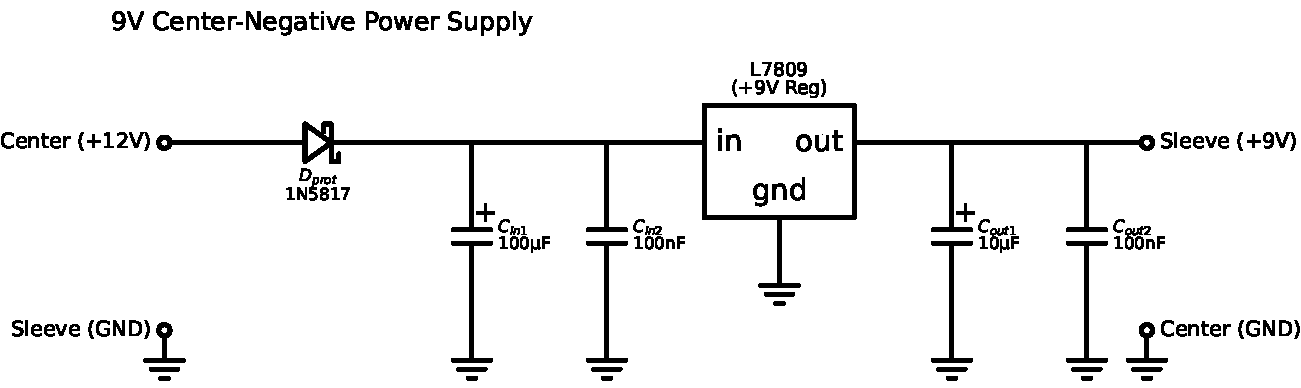
\includegraphics[width=0.8\textwidth]{../power-regulator-12v-to-9v/schematic/exports/power_supply_regulator.pdf}
  \caption{\textbf{Linear Regulator Schematic.} A standard L7809 circuit with input and output bulk capacitance and a reverse-polarity protection diode ($D_{prot}$).}
  \label{fig:power_schematic}
\end{figure}

\section{Thermal Management Strategy}
The main constraint on a linear regulator is heat. The power dissipated ($P_d$) is the voltage drop times the load current:

\begin{equation}
  P_d = (V_{in} - V_{out}) \times I_{load}
\end{equation}

Given an input of $12\text{V}$ and a target output of $9\text{V}$, the regulator drops $3\text{V}$ across the junction.
\begin{itemize}
  \item \textbf{Scenario A (Red Llama):} The analog DUT's current draw was not measured; CMOS pedals of this kind typically draw well under $10\text{mA}$, which would give $P_d < 0.03\text{W}$.
  \item \textbf{Scenario B (Digital Pedals):} Digital reverbs and delays draw far more; a $400\text{mA}$ load is taken as the design case.
\end{itemize}

For Scenario B, the dissipation becomes significant:
\begin{equation}
  P_{max} \approx 3\text{V} \times 0.4\text{A} = 1.2\text{W}
\end{equation}

A standard TO-220 package has a thermal resistance ($\theta_{JA}$) of $\approx 65^\circ \text{C/W}$.\cite{st_l7809cv_datasheet} Without a heatsink, a $1.2\text{W}$ load would result in a temperature rise of:
\begin{equation}
  \Delta T = 1.2\text{W} \times 65^\circ \text{C/W} = 78^\circ \text{C}
\end{equation}
Assuming an ambient temperature of $25^\circ \text{C}$, the silicon junction would reach $103^\circ \text{C}$. That is within the absolute maximum ($125^\circ \text{C}$), but too hot for a closed ABS plastic enclosure.\cite{st_l7809cv_datasheet}

\subsection{The Solution}
Two measures address this:
\begin{enumerate}
  \item \textbf{Conduction:} A bolt-on aluminum heatsink was attached to the TO-220 package to lower the thermal resistance.
  \item \textbf{Convection:} Ventilation holes drilled in the top of the enclosure let warm air rise out, so the insulating ABS box does not trap the heat.
\end{enumerate}

\section{Component Selection}
The BOM, generated with Star Ground, includes these choices for filtering and protection:

\begin{itemize}
  \item \textbf{Input Filtering:} A $100\mu\text{F}$ electrolytic capacitor smooths low-frequency ripple from the 12V source, and a parallel $100\text{nF}$ polyester capacitor filters high-frequency noise.\cite{st_l7809cv_datasheet}
  \item \textbf{Reverse Polarity Protection:} A \textbf{1N5817 Schottky Diode} was selected over a standard 1N4001 silicon diode.\cite{diode_1n5817_datasheet,diode_1n4001_datasheet} The Schottky's lower forward voltage ($V_f \approx 0.45\text{V}$ at its rated $1\text{A}$, and $\approx 0.3\text{V}$ at the few milliamps a pedal draws) leaves more input voltage than a silicon diode ($V_f \approx 0.7\text{V}$).\cite{diode_1n5817_datasheet,diode_1n4001_datasheet}
\end{itemize}

\begin{table}[htbp]
  \centering
  \small\sffamily
  \renewcommand{\arraystretch}{1.4}
  \setlength{\tabcolsep}{4pt}

  % Alternating row colors: starts at row 2, using TableRow gray and white
  \rowcolors{2}{TableRow}{white}

  \begin{tabular}{@{} l l l l r c r l @{}}
    \toprule
    \rowcolor{TableHeader}
    \textbf{\textcolor{white}{Des.}} &
    \textbf{\textcolor{white}{Value}} &
    \textbf{\textcolor{white}{Component}} &
    \textbf{\textcolor{white}{SKU}} &
    \textbf{\textcolor{white}{Price}} &
    \textbf{\textcolor{white}{Qty}} &
    \textbf{\textcolor{white}{Total}} &
    \textbf{\textcolor{white}{Notes}} \\
    \midrule

    U1 & L7809 & L7809CV-DG Reg 9V 1.5A & A-1597 & \$0.25 & 1 & \$0.25 & TO-220 \\
    $D_{prot}$ & 1N5817 & Schottky Diode 1A 20V & A-159 & \$0.06 & 1 & \$0.06 & Low $V_f$ \\
    $C_{in1}$ & $100\mu\text{F}$ & 35V Radial Electrolytic & A-987 & \$0.03 & 1 & \$0.03 & Bulk In \\
    $C_{out1}$ & $10\mu\text{F}$ & 50V Radial Electrolytic & A-4554 & \$0.02 & 1 & \$0.02 & Bulk Out \\
    $C_{f1,f2}$ & 100nF & 100V 5\% Poly Box & A-564 & \$0.10 & 2 & \$0.20 & HF Filter \\
    J1 & 2.1mm & DC Power Jack (Fem) & A-2237 & \$0.13 & 1 & \$0.13 & Panel Mnt \\
    P1 & 2.1mm & DC Plug (Male) Pigtail & A-6806 & \$0.15 & 1 & \$0.15 & Output \\
    -- & Box & Black Plastic Box 03 & A-2383 & \$2.50 & 1 & \$2.50 & ABS \\
    -- & Heatsink & TO-220 10-Fin 1" & A-1512 & \$0.24 & 1 & \$0.24 & For U1 \\
    -- & M3 & Hex Socket Cap Screw & A-6379 & \$0.10 & 1 & \$0.10 & Mounting \\

    \midrule
    \rowcolor{white}
    \multicolumn{6}{r}{\textbf{PROJECT TOTAL}} & \textbf{\$3.68} & \\
    \bottomrule
  \end{tabular}

  \caption{\textbf{Bill of Materials.} All parts were bought from Tayda Electronics to combine shipping. Prices are unit costs at the time of purchase.}
  \label{tab:bom_power}
\end{table}

% =============================================================================
% CHAPTER 4: RED LLAMA
% =============================================================================
\chapter{Device Under Test: Red Llama Overdrive}

\section{Circuit Topology}
With parts ordering (Chapter 2) and power (Chapter 3) in place, work began on the main device: the \textbf{Red Llama Overdrive}.

The circuit is unusual among guitar pedals. Most overdrives use an operational amplifier (op-amp) with clipping diodes in the feedback loop; the Red Llama uses a \textbf{CD4049 CMOS hex inverter} instead.\cite{ti_cd4049ub_datasheet}

The CD4049 is a digital logic chip; each inverter is a complementary pair of MOSFETs in a push-pull arrangement.\cite{ti_cd4049ub_datasheet} Negative feedback biases each inverter into its linear region, where it works as an amplifier. When a guitar signal drives it hard, the output approaches the supply rails along a rounded curve, which is the basis of the comparison with vacuum tubes; at maximum gain the waveform squares off into fuzz.

\section{Procurement \& Fabrication}
The build used the files generated by \textbf{Star Ground}. The ``Field Manual'' PDF set the assembly order by component height, so the low resistors were soldered before the taller IC sockets and capacitors, which made the dense board easier to assemble.

\section{Engineering Deviation: The Diode Mod}
The build follows the standard Way Huge Electronics schematic except for one change to the power section, which raises the supply voltage slightly.

The reference design calls for a \textbf{1N4001} silicon diode at position D2 for reverse-polarity protection.\cite{tayda_redllama_schematic} As noted in Chapter 3, a silicon diode drops $\approx 0.7\text{V}$.\cite{diode_1n4001_datasheet} In a 9V circuit, that is a noticeable loss:

\begin{equation}
  V_{rail} = V_{source} - V_{diode} = 9.0\text{V} - 0.7\text{V} = 8.3\text{V}
\end{equation}

The CD4049's output swing is limited by its supply rails, so losing 0.7V reduces the swing available before clipping. I replaced the 1N4001 with a \textbf{1N5817 Schottky diode}, whose forward drop is $\approx 0.3\text{V}$ at the few milliamps the pedal draws.\cite{diode_1n5817_datasheet}

\begin{equation}
  V_{rail(mod)} = 9.0\text{V} - 0.3\text{V} = 8.7\text{V}
\end{equation}

The extra $\approx 0.4\text{V}$ of supply gives the inverters slightly more output swing before saturation. The effect on the sound was not measured.

\section{The Validation Gap}
Once finished, the pedal powered up without faults and produced sound, and by ear the tone was rich in harmonics. Listening alone, though, says nothing quantitative about how the circuit saturates, so I needed to measure it.

I did not own an oscilloscope. Rather than buying one, I used a spare \textbf{RP2040} microcontroller from the Star Ground order, whose built-in ADC can sample fast enough for audio.\cite{raspberrypi_rp2040_datasheet} This led to the development of the custom DAQ system detailed in the following chapter.

% =============================================================================
% CHAPTER 5: INSTRUMENTATION (RP2040 DAQ)
% =============================================================================
\chapter{Instrumentation: RP2040 DAQ}

\section{System Architecture}
Measuring the Red Llama's saturation (Chapter 4) needs a data acquisition (DAQ) system that captures the full audio band. The \textbf{RP2040} microcontroller (dual-core ARM Cortex-M0+) was chosen for its low cost, built-in ADC and flexible I/O.\cite{rpi_rp2040_datasheet}

The firmware uses a \textbf{store-and-forward} design. Streaming samples over USB while capturing would let USB timing disturb the sampling loop. Instead, the firmware captures a burst into a buffer allocated in RAM at boot, and sends it over USB serial only \textit{after} the capture is complete.\cite{rpi_rp2040_datasheet} The sampling loop's timing is then independent of USB and of the host computer.

\section{Analog Front End (AFE) Theory}
The RP2040's internal ADC is limited to a $0\,\text{V}$ to $3.3\,\text{V}$ unipolar range.\cite{rpi_rp2040_datasheet} The Red Llama's output swings well below 0\,V, so a direct connection would clip the negative half-cycles and risk latch-up in the RP2040. A signal conditioning circuit (the ``universal'' AFE) scales, biases and clamps the signal to fit the ADC's range.

\begin{figure}[htbp]
  \centering
  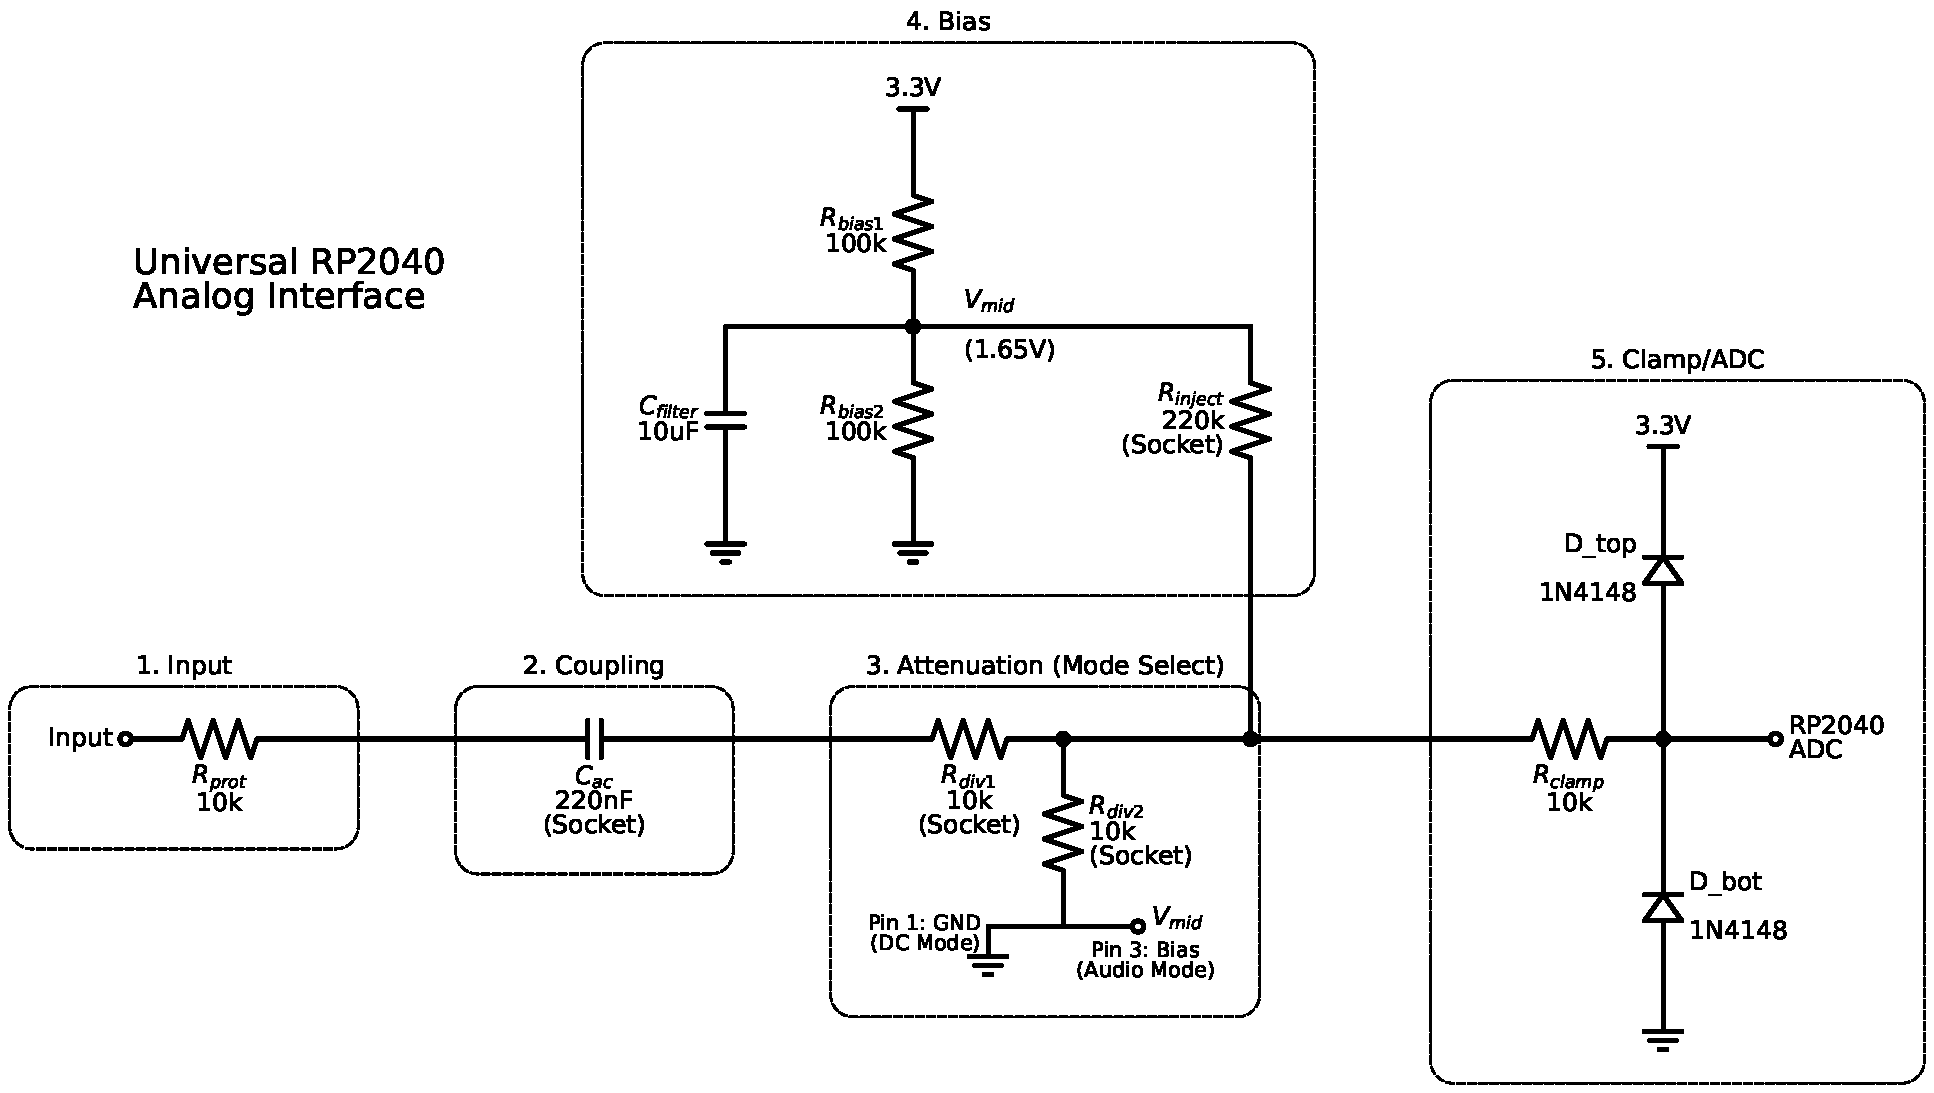
\includegraphics[width=\textwidth]{../oscilloscope-rp2040/schematics/exports/signal_conditioning_universal-blocked.pdf}
  \caption{\textbf{System Schematic.} The signal path flows left-to-right: Protection Stage $\rightarrow$ AC Coupling $\rightarrow$ Attenuation/Bias Network $\rightarrow$ ADC Input.}
  \label{fig:schematic}
\end{figure}

\subsection{Input Protection I}
A series resistor $R_{prot} = 10\,\text{k}\Omega$ is placed immediately at the input jack. It limits the current into the clamping diodes during voltage spikes or an accidental connection to a modular synth power rail ($\pm 12\,\text{V}$), so the diodes are not destroyed.

\subsection{High-Pass Filter (AC Coupling)}
For audio signals, the DC component is blocked using a polyester film capacitor $C_{ac} = 220\,\text{nF}$. The corner frequency ($f_c$) is determined by the input impedance of the subsequent stage.
In \textbf{High-Z / Guitar Mode}, the input impedance is dominated by the bias injection resistor $R_{inject} = 220\,\text{k}\Omega$.

\begin{equation}
  f_c = \frac{1}{2\pi R C} = \frac{1}{2\pi \cdot 220\,\text{k}\Omega \cdot 220\,\text{nF}} \approx 3.29\,\text{Hz}
\end{equation}

The response is therefore flat well below the bottom of the audible range ($20\,\text{Hz}$).

\subsection{Bias \& Switched Reference Topology}
The RP2040 ADC requires a signal centered at $1.65\,\text{V}$ (half-rail) to read AC waveforms.\cite{rpi_rp2040_datasheet} A divider of two $100\,\text{k}\Omega$ resistors, filtered by a $10\,\mu$F electrolytic capacitor, generates this mid-rail voltage ($V_{mid}$).

A jumper (JP1) selects the reference voltage at the bottom of the attenuator (a \textbf{switched reference}). An earlier version tied the attenuator to ground and injected the bias separately, and the divider pulled the bias voltage down:
\begin{itemize}
  \item \textbf{Audio Mode:} The jumper connects the bottom of the attenuation network to $V_{mid}$ ($1.65\,\text{V}$). The divider then attenuates around $V_{mid}$ instead of ground, which keeps the attenuation ratio and biases the signal at the same time.
  \item \textbf{DC Mode:} The jumper connects to GND, forming a standard resistive divider for unipolar sensing ($0-5\,\text{V}$ sensors).
\end{itemize}

\subsection{Clamping \& Safety Analysis (Silicon vs. Schottky)}
The rail clamps use \textbf{1N4148 silicon diodes} rather than the more common Schottky diodes.

Low-voltage input protection often uses Schottky diodes (e.g., BAT54) because their low forward voltage ($V_f \approx 0.3\,\text{V}$) keeps the input within the usual absolute maximum of $V_{DD} + 0.5\,\text{V}$.\cite{nexperia_bat54_datasheet} However, Schottky diodes exhibit significant reverse leakage current ($I_R \approx 1\text{--}5\,\mu\text{A}$).\cite{nexperia_bat54_datasheet} With this AFE's high impedance (the $220\,\text{k}\Omega$ bias injection resistor), a leakage current of just $1\,\mu\text{A}$ would shift the DC level by $V_{err} = 220\,\text{mV}$, a large loss of usable range.

The 1N4148's leakage is far lower ($I_R < 25\,\text{nA}$).\cite{generic_1n4148_datasheet} The trade-off is a higher forward voltage ($V_f \approx 0.7\,\text{V}$).\cite{generic_1n4148_datasheet} During an over-voltage event, the clamping node reaches:
\begin{equation}
  V_{clamp} = V_{DD} + V_f = 3.3\,\text{V} + 0.7\,\text{V} = 4.0\,\text{V}
\end{equation}

This exceeds the RP2040 absolute maximum rating of $3.8\,\text{V}$.\cite{rpi_rp2040_datasheet} The input is instead protected by the current-limiting resistor $R_{clamp}$ ($10\,\text{k}\Omega$). If the external signal forces the node to $4.0\,\text{V}$, the internal ESD diodes of the ADC will begin to conduct at approx $3.8\,\text{V}$. The resulting current injected into the pin is:

\begin{equation}
  I_{inj} = \frac{V_{clamp} - V_{internal}}{R_{clamp}} = \frac{4.0\,\text{V} - 3.8\,\text{V}}{10\,\text{k}\Omega} = 20\,\mu\text{A}
\end{equation}

An injection current of $20\,\mu\text{A}$ is small, so the input relies on current limiting rather than on staying below the voltage rating.

\section{Hardware Configuration}
The board's mode is set by which socketed parts are fitted and the position of the 3-pin jumper, so the same board can serve as a guitar input, a line-level input or a 0--5\,V sensor input.

\begin{table}[htbp]
  \centering
  \small\sffamily
  \renewcommand{\arraystretch}{1.3}
  \rowcolors{2}{TableRow}{white}

  \begin{tabular}{@{} l l l l l @{}}
    \toprule
    \rowcolor{TableHeader}
    \textbf{\textcolor{white}{Mode}} &
    \textbf{\textcolor{white}{Application}} &
    \textbf{\textcolor{white}{Jumper (JP1)}} &
    \textbf{\textcolor{white}{$\mathbf{R_{div1}/R_{div2}}$}} &
    \textbf{\textcolor{white}{$\mathbf{R_{inject}}$}} \\
    \midrule

    Audio (Std)      & Synths, Pedals & Pin 2-3 ($V_{mid}$) & 10k / 10k      & \textit{Empty} \\
    Guitar (High-Z) & Passive Inst.  & Pin 2-3 ($V_{mid}$) & Wire / \textit{Empty} & 220k \\
    DC / Sensor      & 0-5V Signals   & Pin 1-2 (GND)       & 10k / 10k      & \textit{Empty} \\
    \bottomrule
  \end{tabular}

  \caption{Jumper Settings and Component Population Guide}
  \label{tab:config}
\end{table}

\section{Firmware Logic}
The firmware is written in MicroPython for fast development, but interpreted MicroPython is too slow for audio-rate sampling. The capture loop therefore uses the \lstinline|@micropython.native| decorator.\cite{micropython_speed_python}

\begin{lstlisting}[caption=Native Emitter Capture Loop]
@micropython.native
def capture_burst(adc_obj, buf, size: int):
    # Compiles to ARM Thumb machine code
    for i in range(size):
        buf[i] = adc_obj.read_u16()
\end{lstlisting}

This instructs the compiler to emit ARM Thumb machine code directly.\cite{micropython_speed_python} The \texttt{read\_u16()} method lookup still has some overhead, but the loop itself (increment, compare, jump) becomes native CPU instructions. With this the loop reaches $97.69\,\text{kSps}$ (Section~\ref{sec:calibration}), against an initial target of 40\,kSps.

\section{Calibration: Mains Hum and Reference Tones}
\label{sec:calibration}
Frequency-domain analysis needs the sample rate ($F_s$) to be known accurately. The RP2040's clock is stable, but samples are taken by a MicroPython loop on the CPU rather than by a hardware timer with DMA, so the sample rate is set by how long each pass of the loop takes. That time is consistent but not known in advance.

Without a signal generator, the first calibration used the one reference frequency available everywhere: the North American power grid ($60.00\,\text{Hz}$).

\subsection{Physics of Environmental Coupling}
The calibration signal was picked up by touching the input tip, through \textbf{capacitive coupling}. The path can be modeled as a capacitive voltage divider:
\begin{enumerate}
  \item \textbf{Source ($V_{grid}$):} The 120\,V$_{rms}$ wiring in the walls creates an oscillating electric field ($\omega = 2\pi \cdot 60$).
  \item \textbf{Coupling Impedance ($Z_c$):} The user's body acts as a conductive plate separated from the wiring by a dielectric (air/insulation). This forms a stray capacitance ($C_{stray} \approx 10-100$\,pF).
  \item \textbf{Load Impedance ($Z_{in}$):} The AFE input resistance (approx. $220\,\text{k}\Omega$ in High-Z mode).
\end{enumerate}

The voltage at the ADC ($V_{adc}$) is set by the ratio of the input impedance to the total path impedance. The reactance of 50\,pF at 60\,Hz is about $53\,\text{M}\Omega$, so the path attenuates heavily, but the source is large ($\approx 170\,\text{V}_{pk}$), so a signal of a few millivolts still reaches the ADC.

\subsection{Derivation of the Correction Factor}
Because the frequency axis of an FFT scales linearly with $F_s$, a reference of known frequency $f_{ref}$ that measures $f_{meas}$ under an assumed rate $F_{assumed}$ gives the true rate directly:

\begin{equation}
  F_{real} = F_{assumed} \cdot \frac{f_{ref}}{f_{meas}}
\end{equation}

The first-pass calibration applied this to the mains hum, locating the 60\,Hz peak with a weighted average of the FFT bins around it, and gave $F_s = 97{,}859.6$\,Hz (Notebook~\texttt{01}, first cell).

\subsection{Verification Against Crystal-Referenced Tones}
Mains hum is a weak reference for a single burst. The grid wanders by a few hundredths of a hertz, a 16,384-sample burst holds only $\approx 10$ cycles, and the coupled hum is just $2.4$\,mV peak, $2.3$\,dB above the noise floor. The Phase II test tones (Section \ref{sec:transfer}) are a much better reference: a sound card derives them from a crystal clock, typically accurate to $\pm 50$\,ppm. Each was fitted by least squares, which for a steady tone resolves frequency far below the $\approx 6$\,Hz FFT bin (Notebook~\texttt{02}, \S5b):

\begin{table}[htbp]
  \centering
  \small\sffamily
  \renewcommand{\arraystretch}{1.3}
  \rowcolors{2}{TableRow}{white}
  \begin{tabular}{@{} l r r @{}}
    \toprule
    \rowcolor{TableHeader}
    \textbf{\textcolor{white}{Reference}} &
    \textbf{\textcolor{white}{Assumed $F_s$ (Hz)}} &
    \textbf{\textcolor{white}{Implied $F_s$ (Hz)}} \\
    \midrule
    1\,kHz sine, laptop direct      & 97,793.1 & 97,683.3 \\
    1\,kHz sine, via Red Llama      & 97,793.1 & 97,683.2 \\
    100\,Hz triangle, laptop direct & 97,793.1 & 97,688.9 \\
    60\,Hz mains hum                & 97,859.6 & 97,570.3 \\
    \bottomrule
  \end{tabular}
  \caption{Sample rate implied by each reference signal. The statistical bounds of the tone fits ($\le 0.4$\,Hz) are far below the $5.7$\,Hz spread between tones and do not set the uncertainty; the mains fit's bound is $\pm 32$\,Hz. Source: Notebook~\texttt{02}, \S5b.}
  \label{tab:fs}
\end{table}

The three crystal-referenced tones agree within $58$\,ppm. Combined with the sound card's $\pm 50$\,ppm clock tolerance this gives $77$\,ppm, quoted as $F_s = 97.69\,\text{kHz} \pm 0.01\%$. The mains calibration was $0.18\%$ high, and the hardware default used during the Phase II captures ($97{,}793.1$\,Hz) $0.11\%$ high; the mains capture is consistent with the tones within its large uncertainty. All analysis in Chapter 6 uses the measured rate. A rate error scales every frequency axis by the same factor, so harmonic ratios, THD and decibel levels are unaffected by it.

\section{Final Technical Specifications}
Table~\ref{tab:specs} summarizes the measured performance of the finished instrument.

\begin{table}[htbp]
  \centering
  \small\sffamily
  \renewcommand{\arraystretch}{1.3}
  \rowcolors{2}{TableRow}{white}

  \begin{tabular}{@{} l l @{}}
    \toprule
    \rowcolor{TableHeader}
    \textbf{\textcolor{white}{Parameter}} &
    \textbf{\textcolor{white}{Value / Note}} \\
    \midrule

    \textbf{ADC Resolution}       & 12-bit (Scaled to 16-bit integer) \\
    \textbf{Sample Rate ($F_s$)} & $97.69\,\text{kHz} \pm 0.01\%$ (Crystal-referenced) \\
    \textbf{Bandwidth}           & DC -- 48.8\,kHz (Nyquist Limit) \\
    \textbf{Buffer Depth}        & 16,384 Samples ($\approx 168$\,ms duration) \\
    \textbf{Stream Mode}         & 1,024-sample blocks; $\approx 75\%$ duty cycle (untimed gaps) \\
    \textbf{Spectral Resolution} & $5.96\,\text{Hz}$ per FFT bin \\
    \textbf{Input Range}         & 0--3.3\,V (Unipolar) / $\pm 3.3$\,V (AC Coupled) \\
    \textbf{Noise Floor}         & $1.29\,\text{mV}$ RMS (input open) \\
    \textbf{Dynamic Range}       & $59.1\,\text{dB}$ full-scale sine to noise ($9.5$ effective bits) \\
    \bottomrule
  \end{tabular}

  \caption{Measured System Performance. Source: Notebook~\texttt{02}, \S5b (sample rate), Notebook~\texttt{02}, \S5 (noise floor, dynamic range), Notebook~\texttt{04}, \S3 (stream-mode duty cycle); bandwidth, buffer duration and bin width follow from $F_s$ and $N$.}
  \label{tab:specs}
\end{table}

% =============================================================================
% CHAPTER 6: SYSTEM INTEGRATION & ANALYSIS
% =============================================================================
\chapter{Analysis \& Validation}

\section{Experimental Methodology}
For the guitar measurements, the Red Llama was connected between an electric guitar (neck pickup) and the RP2040 DAQ. Each capture used the firmware's ``science mode,'' a gap-free burst of $N=16,384$ samples at the calibrated rate of $F_s = 97.69\,\text{kSps}$ (Section \ref{sec:calibration}).

The analysis is written in Python with \texttt{numpy} and \texttt{scipy.signal}.\cite{scipy_signal_tutorial,numpy_fft_fft} To reduce spectral leakage from the finite capture length, a \textbf{Hann window} ($w(n) = 0.5 - 0.5\cos(\frac{2\pi n}{N-1})$) is applied to each buffer before the fast Fourier transform (FFT).\cite{scipy_fft_tutorial, scipy_hann_window} This keeps the side lobes of the strong fundamental from hiding the weaker harmonics.\cite{harris1978_windows_dft}

The swept measurements of Section \ref{sec:transfer} additionally use the firmware's stream mode, which requires a different analysis method described there.

\section{DAQ Sensitivity \& Noise Floor}
Before measuring the DUT, the instrument itself was measured to find its noise floor and dynamic range. Figure \ref{fig:noise} shows its spectrum with the input open.

With the input open, the system exhibits a read noise of $1.293$\,mV RMS, about $1.6$ ADC steps. An independent estimate comes from the mains-hum calibration capture: after fitting and removing the hum, the residual ``thickness'' of the waveform is $1.306$\,mV RMS, agreeing within $1\%$.

The instrument's \textbf{dynamic range} is the ratio of the largest signal it can capture without clipping to its noise floor. The ADC window ($0$--$3.3$\,V) admits a full-scale sine of $1.65$\,V peak, i.e. $1.167\,\text{V}_{rms}$:

\begin{equation}
  \text{DR}_{dB} = 20 \cdot \log_{10}\left(\frac{V_{FS,rms}}{V_{noise,rms}}\right) = 20 \cdot \log_{10}\left(\frac{1.167}{1.293\times10^{-3}}\right) \approx 59.1\,\text{dB}
\end{equation}

This corresponds to $9.5$ effective bits of the ADC's 12 (an ideal 12-bit converter reaches $74.0$\,dB). Mains pickup is negligible: the open-input spectrum contains a 60\,Hz line of only $0.094$\,mV amplitude. All values are computed in Notebook~\texttt{02}, \S5.

\begin{figure}[htbp]
  \centering
  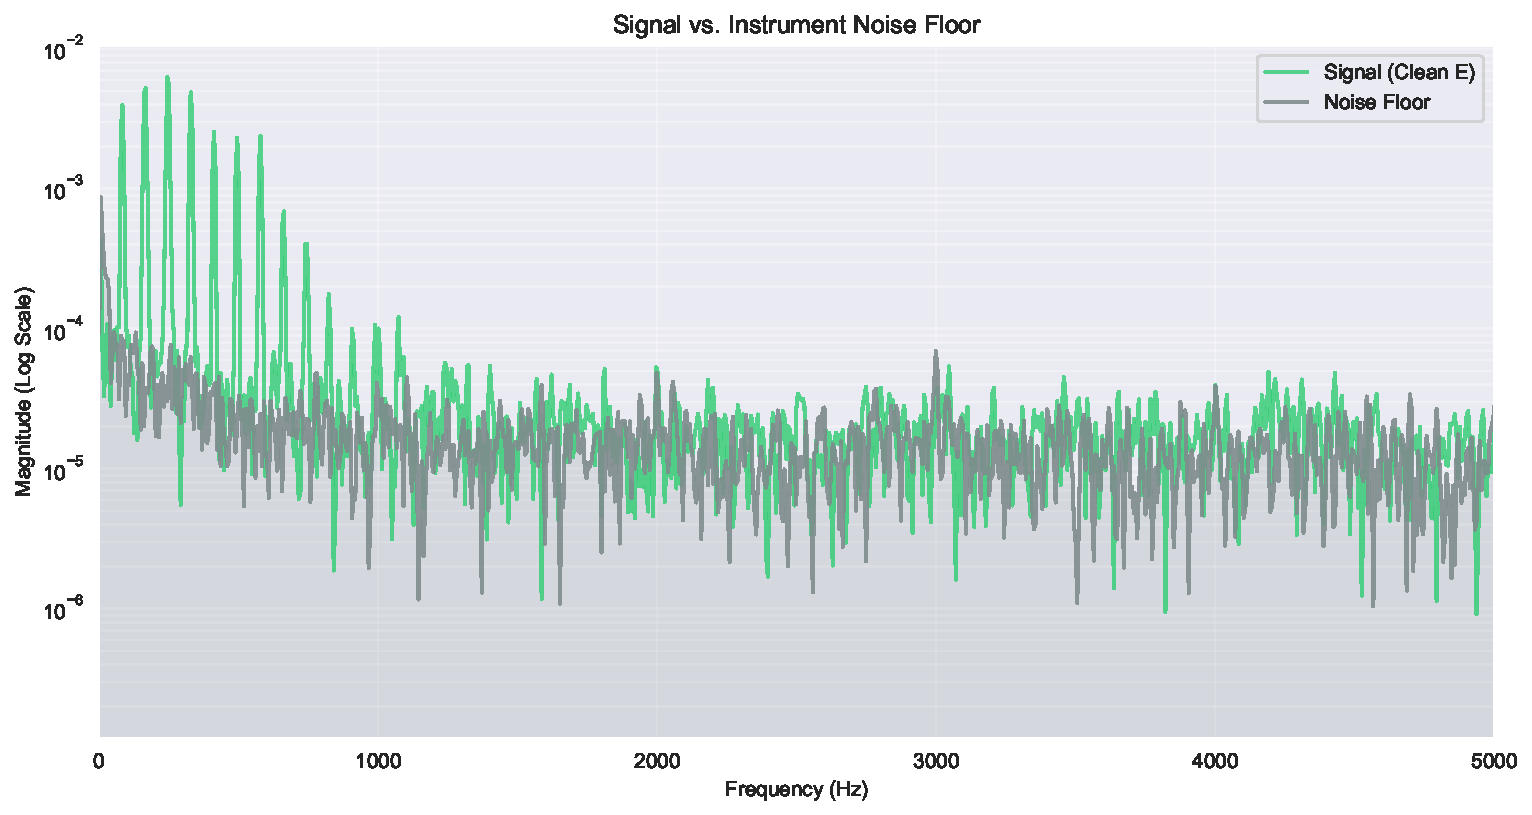
\includegraphics[width=0.9\textwidth]{figures/fig_validation_noise.pdf}
  \caption{\textbf{DAQ Sensitivity Analysis.} Read noise is $1.29\text{mV}$ RMS, and the full-scale dynamic range is $59.1\text{dB}$. Below $1\text{kHz}$ the signal (green) sits well clear of the noise floor (gray). Source: Notebook~\texttt{02}, \S5.}
  \label{fig:noise}
\end{figure}

\section{Gain Structure \& Transfer Characteristic}
\label{sec:gain}
The Red Llama is a high-gain preamplifier. Figure \ref{fig:gain} plots the input signal ($49\text{mV}_{pp}$) and the output on the same voltage scale. The clean note was captured at $1.0\times$ DAQ gain and the Red Llama output through the $0.5\times$ divider; both are referred to the instrument / pedal output.

The output reaches $3.54\text{V}_{pp}$, a peak-to-peak gain of $\approx 72\times$ ($37.1\text{dB}$; Notebook~\texttt{02}, \S3). The figure is approximate: the clean and Red Llama captures are separate plucks, and the divider ratio is nominal.

\subsection{The Saturation Gradient}
The shape of the output waveform reflects how the distortion arises. Plotting $V_{out}$ against $V_{in}$ gives the device's \textbf{transfer characteristic}.
\begin{itemize}
  \item \textbf{High-Gain Region:} Around zero, the output changes steeply with the input.
  \item \textbf{Saturation Region:} As the output approaches its limits, the slope $dV_{out}/dV_{in}$ falls toward zero continuously, without a sharp corner.
\end{itemize}

This is what distinguishes the CMOS circuit from silicon diode clipping. A silicon diode clipper turns into saturation over a narrow band around its forward voltage ($V_f$), giving a sharp knee; the CMOS inverter instead follows a smooth, sigmoid-shaped curve (asymmetric, as Section~\ref{sec:transfer} shows), resulting in a gentler transition into saturation.

\begin{figure}[htbp]
  \centering
  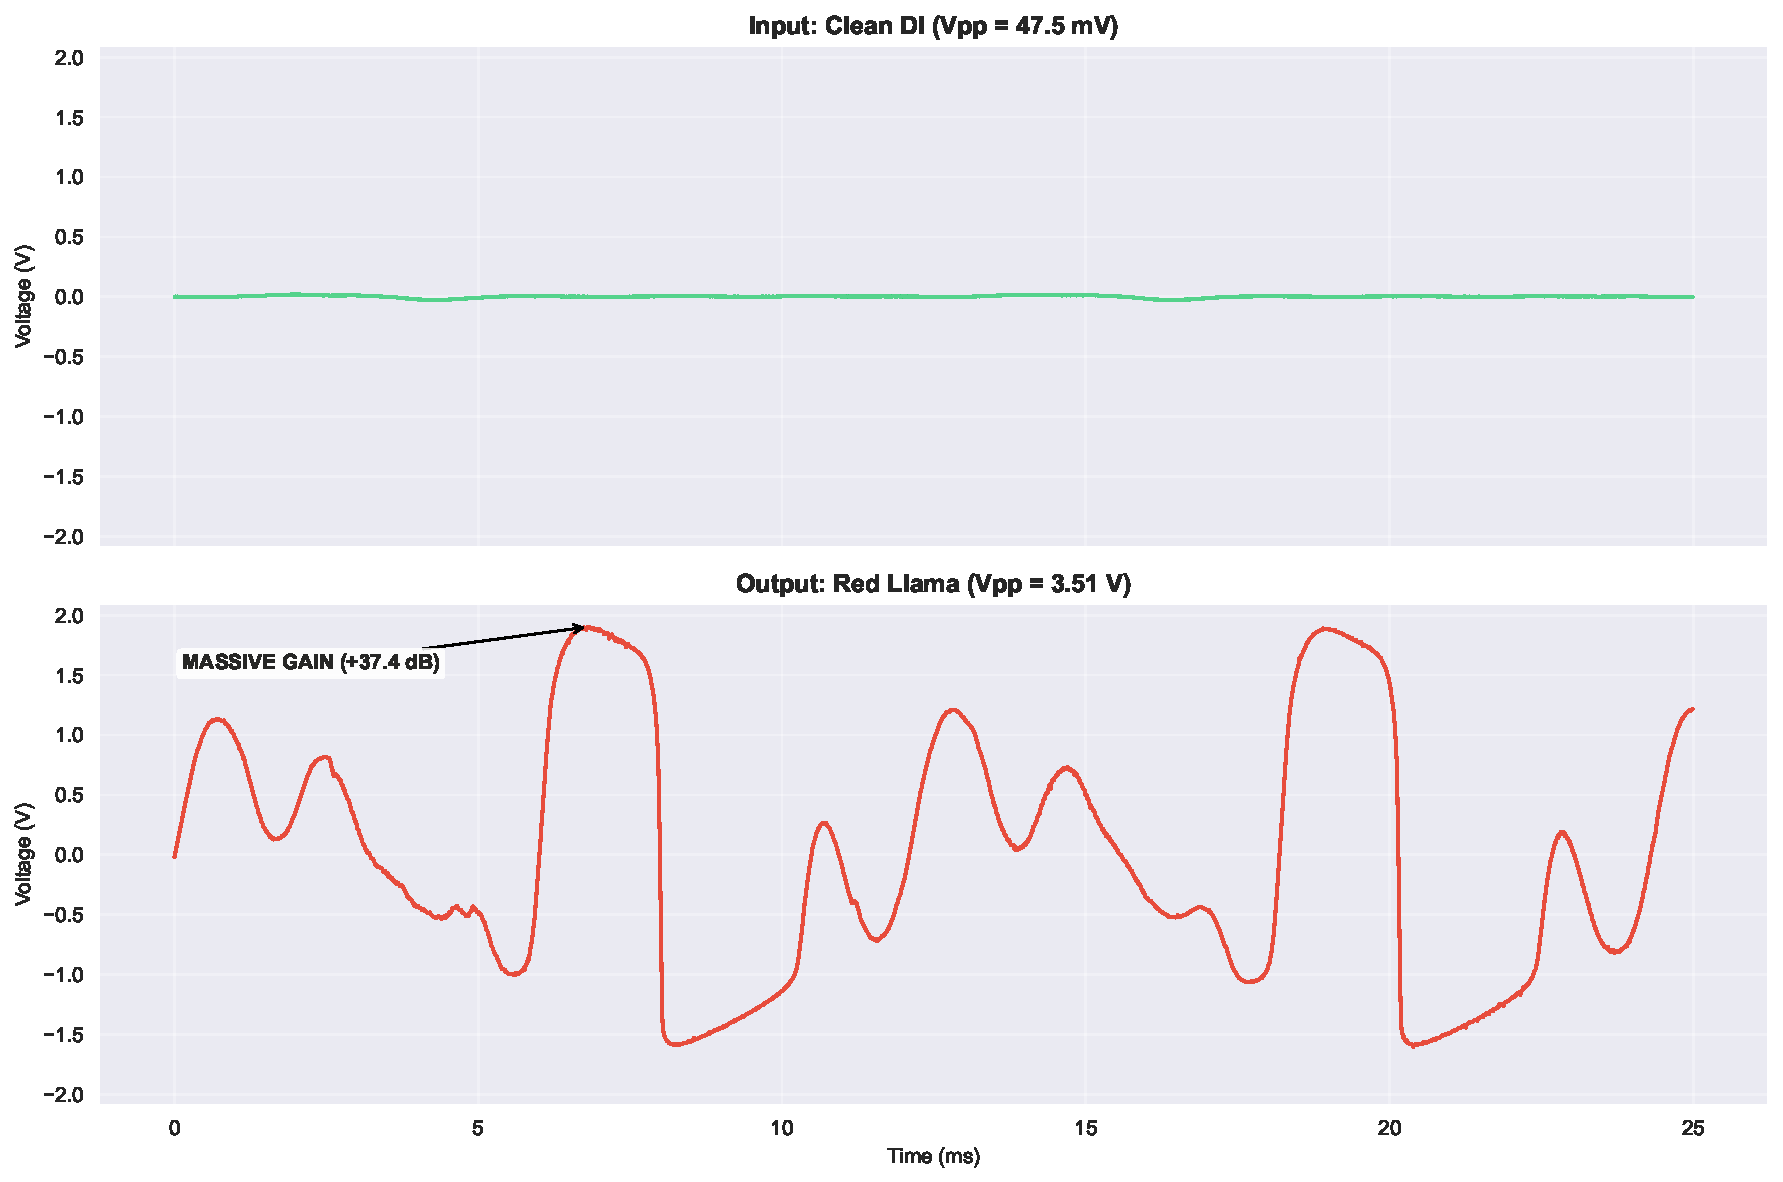
\includegraphics[width=0.9\textwidth]{figures/fig_llama_gain.pdf}
  \caption{\textbf{Gain Stage Characterization.} The circuit provides $\approx 37\text{dB}$ of gain. The squared-off output shows heavy saturation, where the inverters' outputs approach the supply rails. Source: Notebook~\texttt{02}, \S4; over the plotted 25\,ms window the gain is $37.4\text{dB}$.}
  \label{fig:gain}
\end{figure}

\section{Topology \& Harmonic Fingerprint}
\label{sec:topology}
The main hypothesis was that the CD4049, though a digital logic chip, behaves like a vacuum tube triode when biased into its linear region: soft saturation with asymmetric clipping, which favours even-order harmonics. Figure \ref{fig:topology} compares the clean and driven signals after phase alignment.

\subsection{Time Domain: The Soft Knee}
In the left panel of Figure \ref{fig:topology}, the waveform peaks show ``soft knee'' compression, consistent with the smooth transfer characteristic of Section \ref{sec:gain}: the peaks are rounded rather than cut flat. Soft clipping of this kind is usually credited with letting the player control the amount of distortion by how hard they pick, though that was not tested here.

\subsection{Frequency Domain: An Even-Order Shift}
The harmonic analysis (Figure \ref{fig:topology}, Right; Notebook~\texttt{02}, \S7) compares the clean guitar note with the Red Llama output.
\begin{itemize}
  \item \textbf{Even Harmonics ($2^{nd}, 4^{th}$):} The circuit raises $H_2$ from $1.47$ to $2.21$ times the fundamental, making it the strongest component of this capture. Even harmonics arise from asymmetric clipping, the mechanism usually associated with the ``warmth'' of single-ended tube stages.
  \item \textbf{Odd Harmonics ($3^{rd}, 5^{th}$):} $H_3$ falls from $1.73$ to $1.31$. The odd series remains substantial.
\end{itemize}

The guitar note is already rich in harmonics, and the two captures are separate plucks, so this comparison overstates the effect. The pure-tone measurements in Section~\ref{sec:evenodd} give the circuit's own, more modest, even-order bias.

Resolving these harmonic peaks needs the long, gap-free burst: at $5.96\,\text{Hz/bin}$ they are well separated, which the 1,024-sample live view could not achieve.

\begin{figure}[htbp]
  \centering
  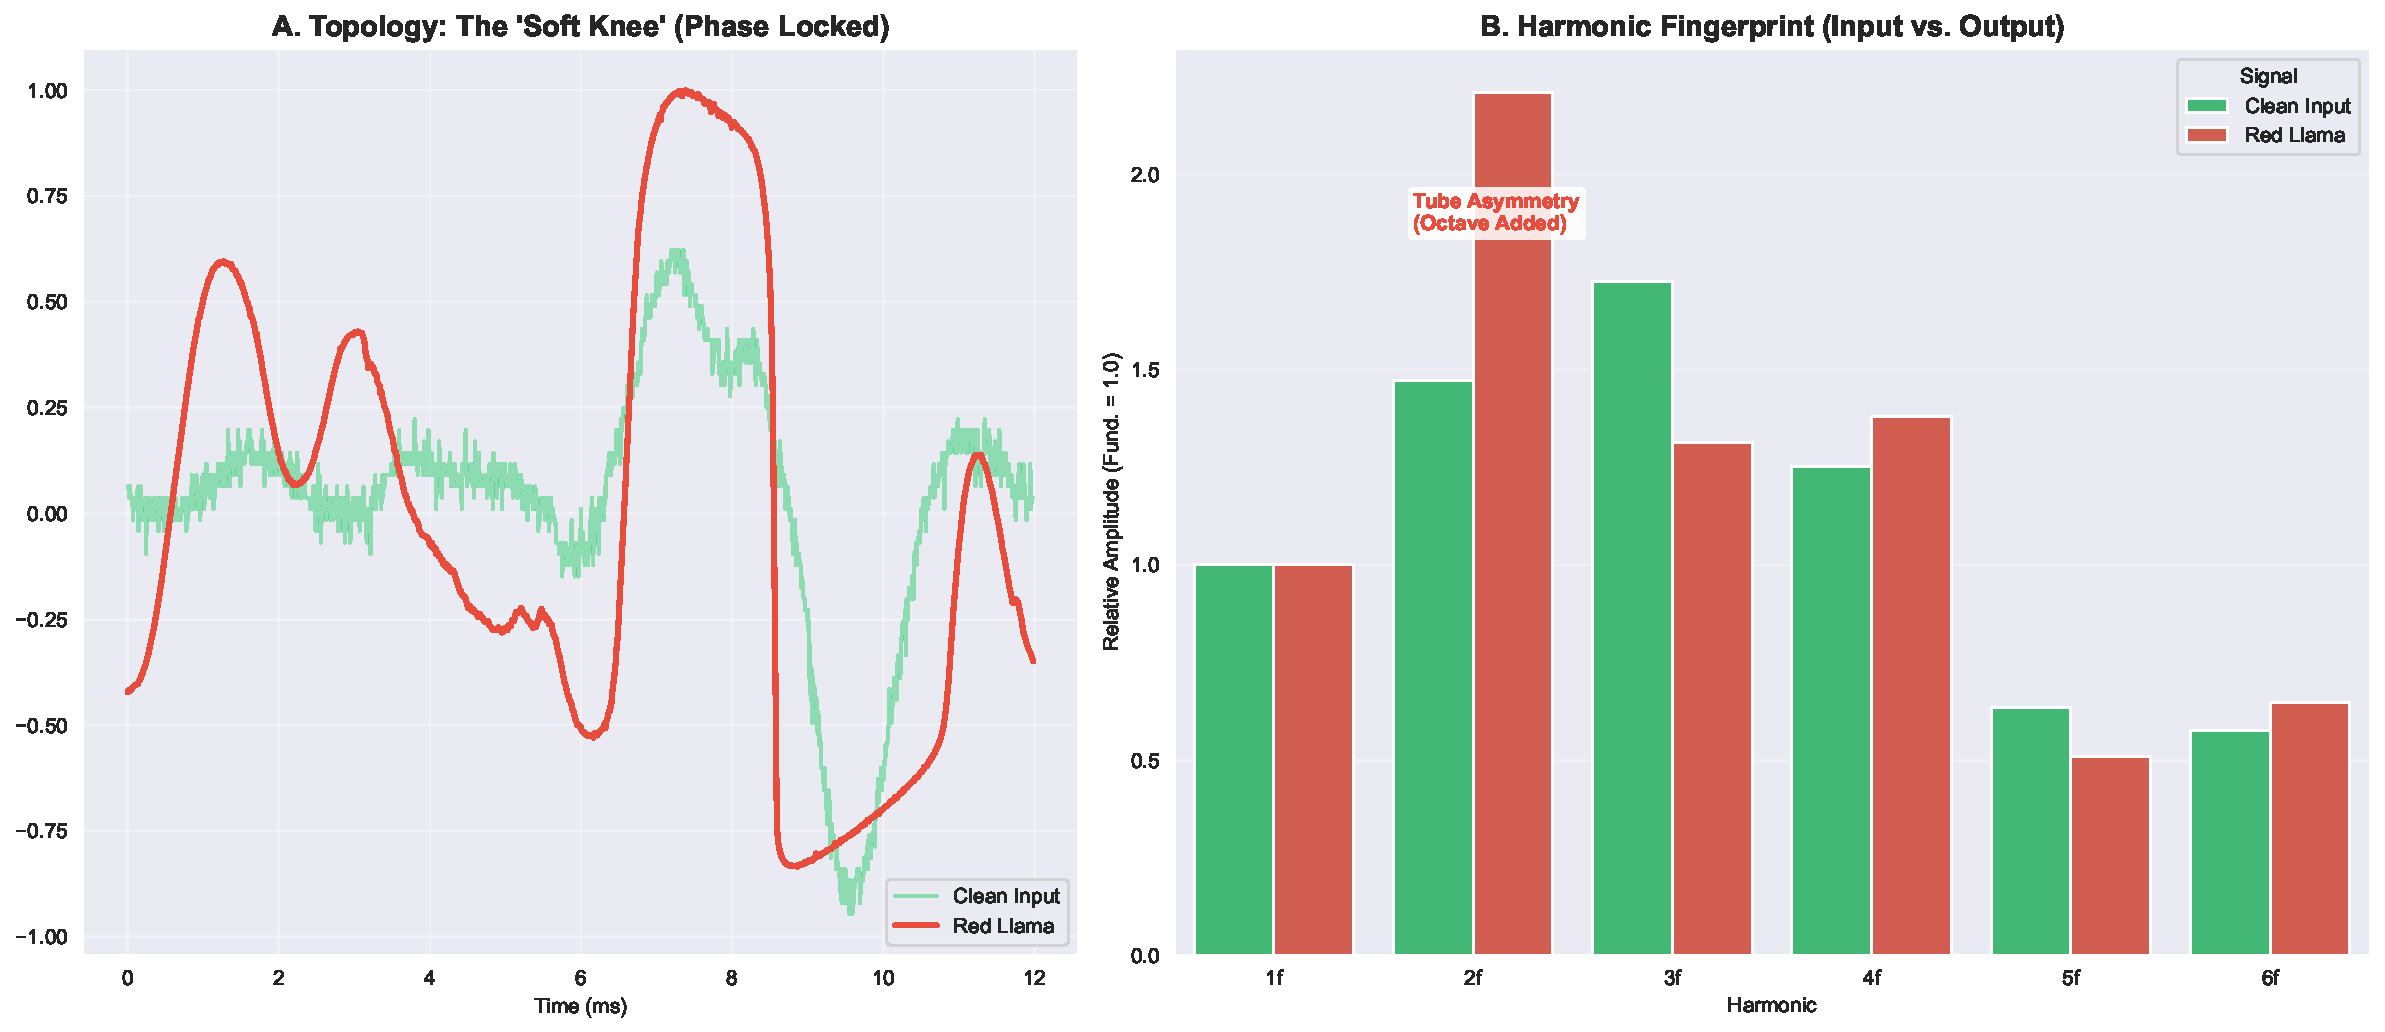
\includegraphics[width=1.0\textwidth]{figures/fig_analysis_topology.pdf}
  \caption{\textbf{Empirical Validation of CMOS Topology.} (A) Phase-aligned time-domain comparison showing ``soft knee'' compression, distinct from hard diode clipping. (B) Harmonic fingerprinting shows the circuit shifting the guitar's harmonics towards even orders ($H_2$ up, $H_3$ down), consistent with asymmetric saturation. Source: Notebook~\texttt{02}, \S9.}
  \label{fig:topology}
\end{figure}

\section{Active Signal Injection: Transfer Function Analysis}
\label{sec:transfer}
The guitar captures measure the DUT at a single, uncontrolled operating point. To measure it across frequency, the laptop's audio output was used as a signal generator, driving the DUT through a TRS-to-TS adapter cable. Four captures were taken (Table \ref{tab:stimuli}).

\begin{table}[htbp]
  \centering
  \small\sffamily
  \renewcommand{\arraystretch}{1.3}
  \rowcolors{2}{TableRow}{white}
  \begin{tabular}{@{} l l l l @{}}
    \toprule
    \rowcolor{TableHeader}
    \textbf{\textcolor{white}{Capture}} &
    \textbf{\textcolor{white}{Stimulus}} &
    \textbf{\textcolor{white}{Signal Path}} &
    \textbf{\textcolor{white}{DAQ Mode}} \\
    \midrule
    Source sweep & Log sweep, 20\,Hz--20\,kHz, 5\,s & Laptop $\to$ DAQ (loopback) & Stream \\
    DUT sweep    & Log sweep, 20\,Hz--20\,kHz, 5\,s & Laptop $\to$ Red Llama (max gain) $\to$ DAQ & Stream \\
    Triangle     & 100\,Hz triangle & Source and DUT captured separately & Burst \\
    Sine         & 1\,kHz sine & Laptop $\to$ Red Llama $\to$ DAQ & Burst \\
    \bottomrule
  \end{tabular}
  \caption{Active signal injection captures. Source: Notebook~\texttt{03} (acquisition), Notebook~\texttt{04}, \S2.}
  \label{tab:stimuli}
\end{table}

\subsection{The Stream-Mode Discontinuity Problem}
A 5\,s sweep does not fit in the 16,384-sample ($\approx 168$\,ms) burst buffer, so the sweeps were captured in the firmware's stream mode. Stream mode is request--response: the host requests a 1,024-sample block, the RP2040 samples it ($10.5$\,ms), transmits it over USB, and waits for the next request. Analysis of the captures shows a block period of $\approx 13.9$\,ms, so roughly 25\% of wall-clock time falls into untimed gaps between blocks. Concatenated, the blocks form a signal with a phase discontinuity at every block boundary (sample-to-sample jumps $100$--$166\times$ larger than elsewhere; Notebook~\texttt{04}, \S3).

The standard technique for swept-sine measurement, Exponential Sine Sweep (ESS) deconvolution,\cite{farina2000_swept_sine} convolves the whole response with an inverse sweep and therefore requires a phase-continuous recording. With 357 untimed gaps it is not applicable to these captures.

\subsection{Chunked Harmonic Fitting}
Although the capture as a whole is discontinuous, each block is gap-free, and a 5\,s log sweep is quasi-stationary over $10.5$\,ms (the frequency changes by $<1.5\%$ within a block; Notebook~\texttt{04}, \S3). The analysis therefore treats each block as a separate measurement:

\begin{enumerate}
  \item \textbf{Timing Recovery.} The sweep's instantaneous frequency is $f(t) = f_1 R^{t}$ with $R = (f_2/f_1)^{1/T}$. The dominant frequency of each block (from a zero-padded, Hann-windowed FFT) implies a sweep time $t_k$. A robust line fit $t_k = t_0 + k\Delta$ recovers the block period ($\Delta = 13.88$\,ms source, $14.03$\,ms DUT; Notebook~\texttt{04}, \S3) and extrapolates to low-frequency blocks where a direct estimate is unreliable.
  \item \textbf{Harmonic Model.} With $\tau$ the time from the block centre and $f_k$ its centre frequency, the exact sweep phase is
    \begin{equation}
      \phi_k(\tau) = \frac{2\pi f_k}{\ln R}\left(R^{\tau} - 1\right),
    \end{equation}
    and each block is fitted by linear least squares to
    \begin{equation}
      x(\tau) = c_0 + \sum_{h=1}^{5} \left[a_h \cos\left(h\,\phi_k(\tau)\right) + b_h \sin\left(h\,\phi_k(\tau)\right)\right],
    \end{equation}
    giving the amplitude of harmonic $h$ as $A_h = \sqrt{a_h^2 + b_h^2}$.
  \item \textbf{Normalization.} The DUT/source ratio of fundamental amplitudes cancels the response of the laptop DAC and the DAQ front end. The source capture's own harmonics define the distortion floor of the measurement chain.
\end{enumerate}

Blocks holding less than one cycle ($f < f_s/1024 \approx 95$\,Hz) are excluded. The method was verified against synthetic stream captures with random gaps and timing jitter, recovering a known first-order low-pass response within $0.5$\,dB and the analytic harmonics of a polynomial nonlinearity within $1$\,dB (\texttt{tests/test\_chunked\_sweep.py}). The implementation is \texttt{sysaudio.chunked\_sweep} (Appendix \ref{app:chunked}).

\subsection{Frequency Response}
The DUT is flat within $0.5$\,dB from $97$\,Hz to $3.4$\,kHz, then rolls off gently: $-1$\,dB at $5.8$\,kHz, $-2$\,dB at $11.9$\,kHz and $-2.8$\,dB at $19.1$\,kHz (Figure \ref{fig:transfer_bode}, top; Notebook~\texttt{04}, \S4). The shallow slope is consistent with a single-pole low-pass formed by the inverters' feedback network, with its corner near the top of the audio band.

This measurement was made at maximum gain, where the circuit is heavily saturated. A saturated stage's output level is set largely by its clipping ceiling rather than by its input, which tends to flatten the apparent response. The small-signal response, including the low-frequency corner of the coupling capacitors (below the $\approx 95$\,Hz analysis floor), remains to be measured at low gain.

\subsection{Harmonic Distortion vs. Frequency}
The harmonic profile is essentially independent of frequency up to $\approx 5$\,kHz (Figure \ref{fig:transfer_bode}, bottom; Notebook~\texttt{04}, \S4): median levels over 200\,Hz--5\,kHz are $H_2 = -12.9$, $H_3 = -12.8$, $H_4 = -15.3$ and $H_5 = -23.7$\,dBc. $H_2$ and $H_3$ are equal, but $H_4$ sits $8$\,dB above $H_5$, an early sign that the series is not symmetric (Section \ref{sec:evenodd}). Above $5$\,kHz the harmonics themselves fall into the treble roll-off, and $H_2$ drops to $-18.3$\,dBc at $19.1$\,kHz. The source loopback's harmonics sit at $\approx -47$\,dBc throughout, more than $30$\,dB below the DUT's, confirming that the measured distortion is produced by the Red Llama and not by the measurement chain.

\begin{figure}[htbp]
  \centering
  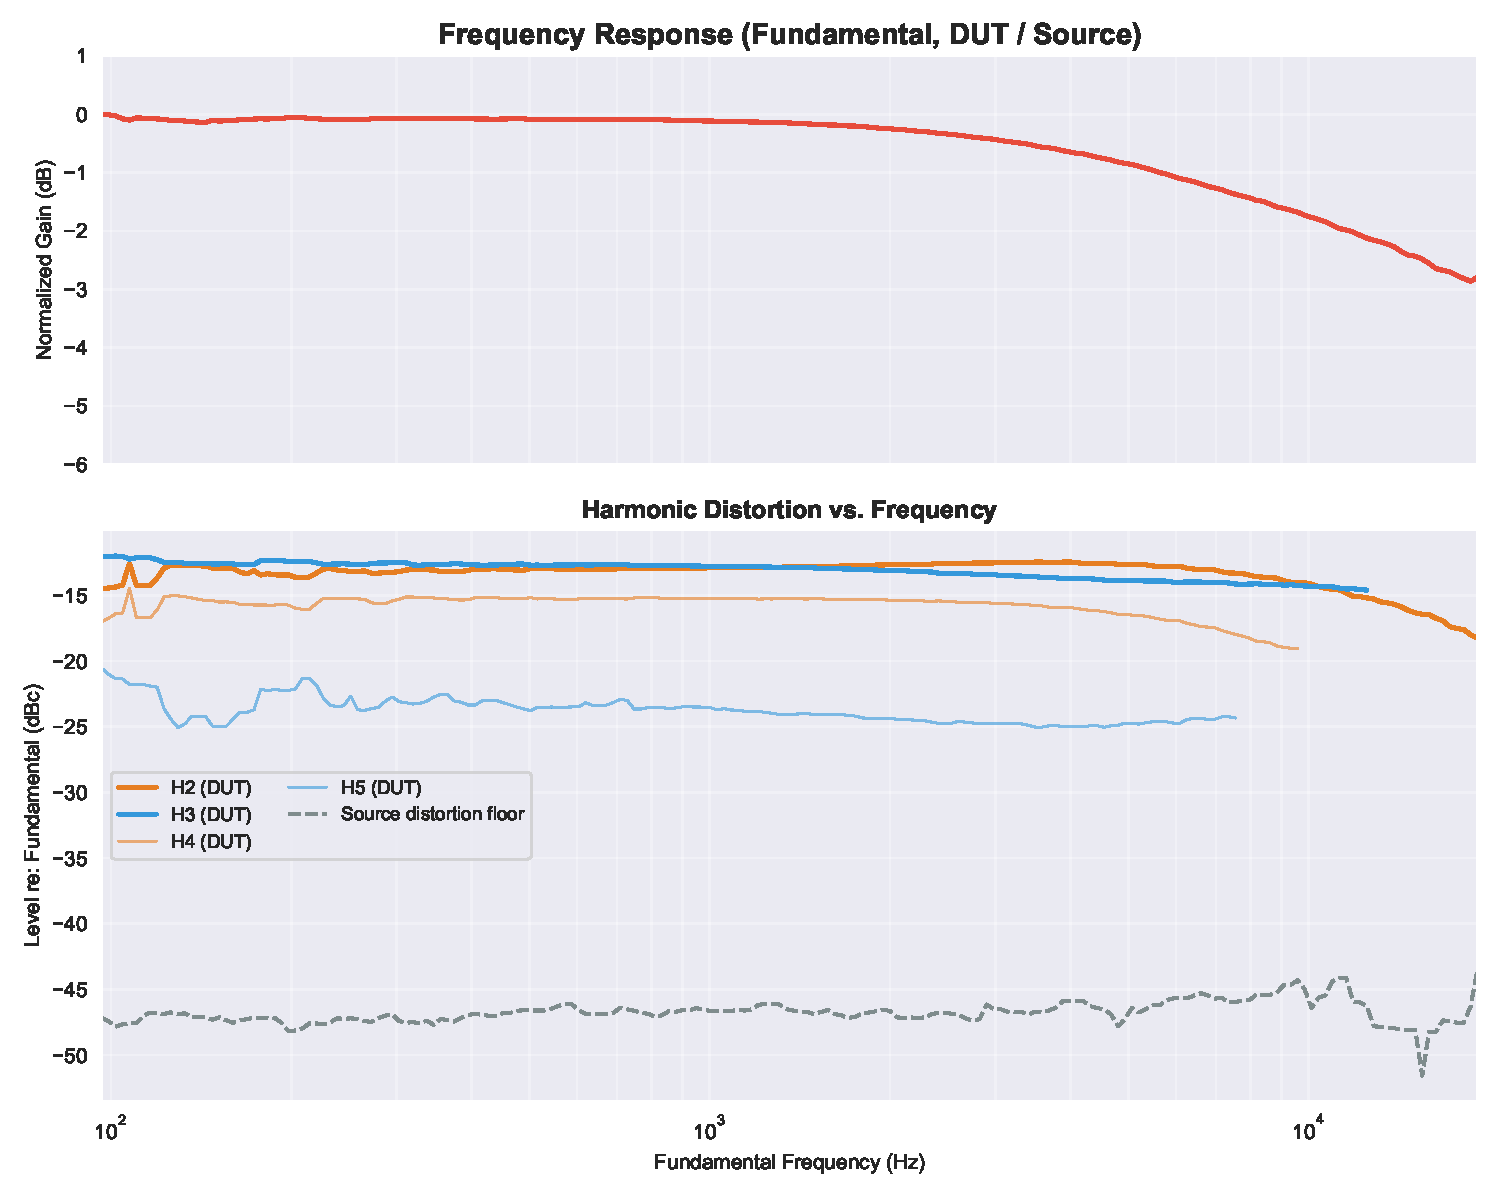
\includegraphics[width=0.9\textwidth]{figures/fig_transfer_bode.pdf}
  \caption{\textbf{Swept Transfer Function (Max Gain).} Top: fundamental magnitude response, DUT/source, normalized to 0\,dB. Bottom: harmonics 2--5 relative to the fundamental, against the source loopback's distortion floor (dashed). Recovered from stream-mode captures by chunked harmonic fitting. Source: Notebook~\texttt{04}, \S4.}
  \label{fig:transfer_bode}
\end{figure}

\subsection{Large-Signal Transfer Curve}
Plotting output against input for a $100$\,Hz triangle (Figure \ref{fig:transfer_curve}; Notebook~\texttt{04}, \S5) traces the saturation curve directly. Its shape refines the earlier findings in three ways:
\begin{itemize}
  \item \textbf{Soft Saturation:} Gain is steep around zero and decreases smoothly toward the rails, with no sharp clipping threshold.
  \item \textbf{Asymmetry:} The pedal output peaks at $+2.11$\,V but only $-1.81$\,V (ratio $1.17$; $1.35$ for the 1\,kHz sine), referred through the DAQ's $0.5\times$ divider. Unequal clipping of the two half-cycles is the physical origin of the even harmonics.
  \item \textbf{Memory:} The rising and falling halves trace different paths, forming a loop rather than a single curve. The coupling capacitors add phase shift at $100$\,Hz, visible as ``droop'' on the flat tops. Part of the loop may be residual misalignment, since source and DUT were captured separately.
\end{itemize}

\begin{figure}[htbp]
  \centering
  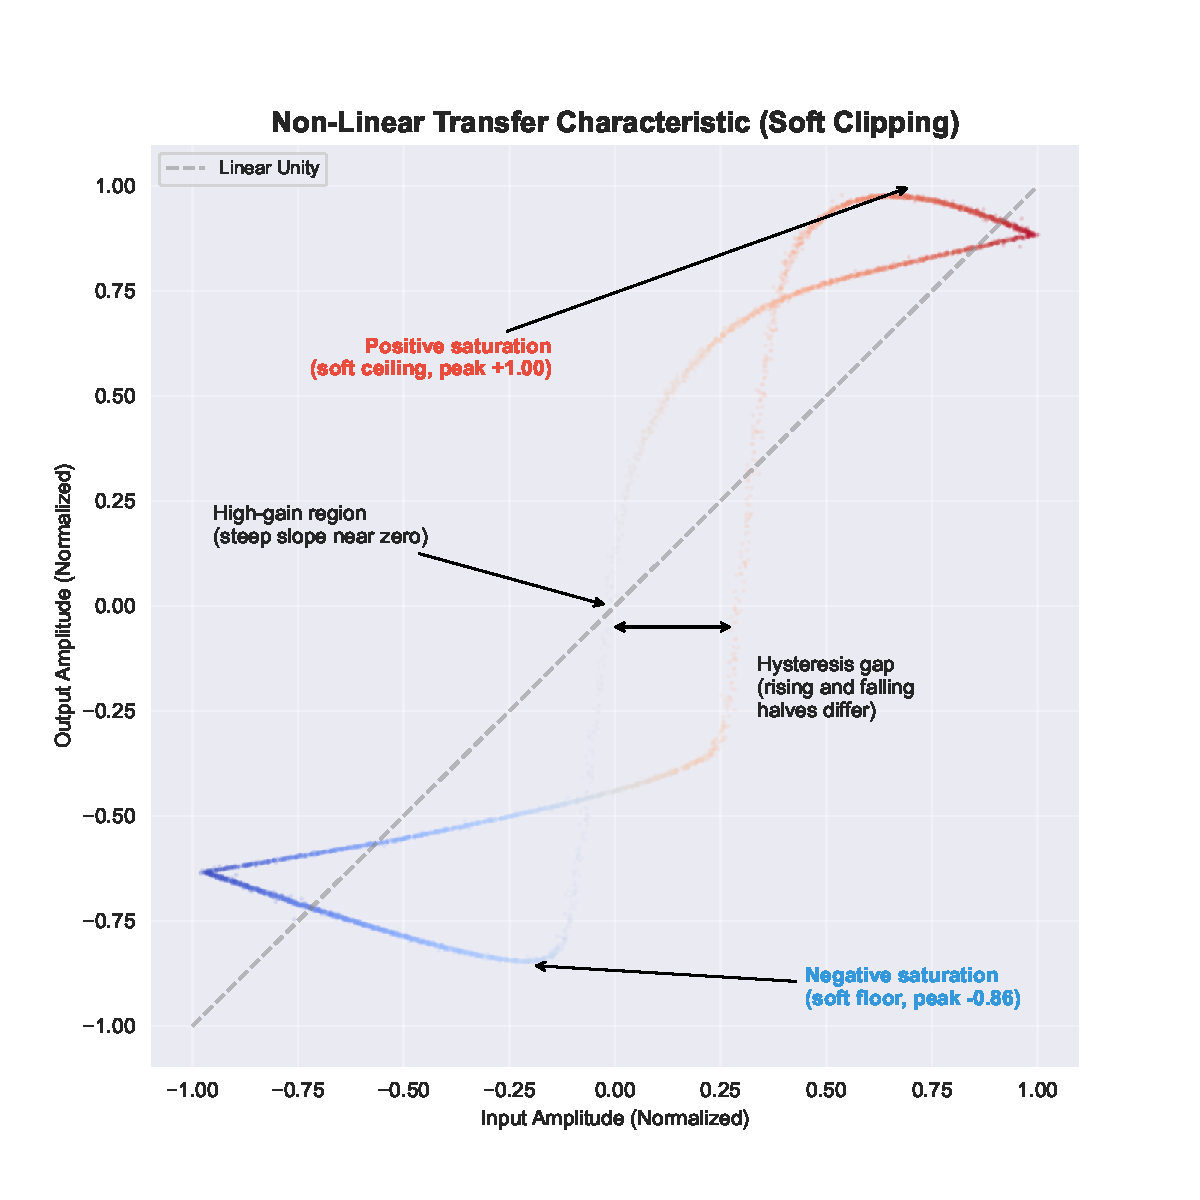
\includegraphics[width=0.6\textwidth]{figures/fig_transfer_curve.pdf}
  \caption{\textbf{Large-Signal Transfer Characteristic.} DUT output vs.\ source input for a 100\,Hz triangle, both normalized. The sigmoid is asymmetric and opens into a loop due to capacitive coupling. Source: Notebook~\texttt{04}, \S5.}
  \label{fig:transfer_curve}
\end{figure}

\subsection{Cross-Validation Against Burst Capture}
A 1\,kHz sine captured in burst mode is gap-free and independent of the sweep analysis. Its harmonic spectrum agrees with the chunked sweep at 1\,kHz to within $0.2$\,dB (Table \ref{tab:crosscheck}, Figure \ref{fig:thd}; Notebook~\texttt{04}, \S6), validating the method on real data.

\begin{table}[htbp]
  \centering
  \small\sffamily
  \renewcommand{\arraystretch}{1.3}
  \rowcolors{2}{TableRow}{white}
  \begin{tabular}{@{} l r r @{}}
    \toprule
    \rowcolor{TableHeader}
    \textbf{\textcolor{white}{Harmonic}} &
    \textbf{\textcolor{white}{Burst Sine (dBc)}} &
    \textbf{\textcolor{white}{Chunked Sweep (dBc)}} \\
    \midrule
    $H_2$ & $-12.9$ & $-12.9$ \\
    $H_3$ & $-12.8$ & $-12.8$ \\
    $H_4$ & $-15.2$ & $-15.2$ \\
    $H_5$ & $-23.7$ & $-23.5$ \\
    \bottomrule
  \end{tabular}
  \caption{Harmonic levels at 1\,kHz from two independent capture modes. Source: Notebook~\texttt{04}, \S6.}
  \label{tab:crosscheck}
\end{table}

\begin{figure}[htbp]
  \centering
  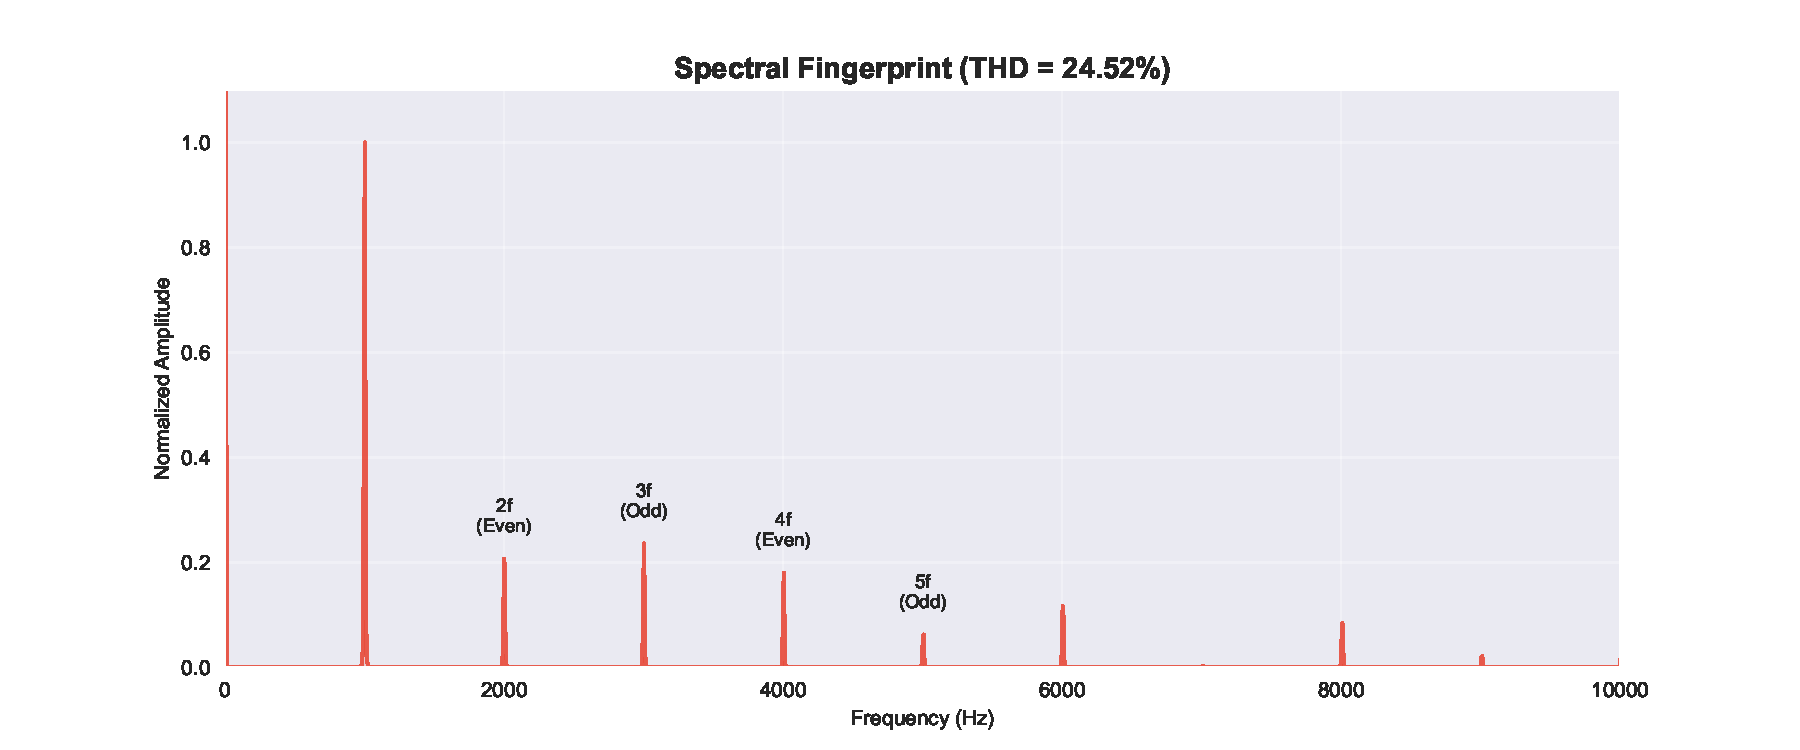
\includegraphics[width=0.9\textwidth]{figures/fig_thd_fingerprint.pdf}
  \caption{\textbf{Steady-State Harmonic Fingerprint at 1\,kHz.} Burst-mode capture of the DUT driven by a 1\,kHz sine. $H_2$ and $H_3$ are equal, while the higher even harmonics ($4f$, $6f$, $8f$) outlast the odd ones ($5f$, $7f$). Source: Notebook~\texttt{04}, \S6.}
  \label{fig:thd}
\end{figure}

\subsection{Even vs. Odd Harmonic Balance}
\label{sec:evenodd}
Comparing $H_2$ with $H_3$ alone hides the shape of the full series. Table \ref{tab:evenodd} gives the ratio of even-order ($H_2, H_4, \dots$) to odd-order ($H_3, H_5, \dots$) harmonic energy over $H_2$--$H_8$, computed in Notebook~\texttt{02}, \S7 (guitar) and Notebook~\texttt{04}, \S6 (1\,kHz sine) with a common method (measured fundamental, main-lobe energy, local noise floor removed).

\begin{table}[htbp]
  \centering
  \small\sffamily
  \renewcommand{\arraystretch}{1.3}
  \rowcolors{2}{TableRow}{white}
  \begin{tabular}{@{} l r r @{}}
    \toprule
    \rowcolor{TableHeader}
    \textbf{\textcolor{white}{Stimulus}} &
    \textbf{\textcolor{white}{Clean Input}} &
    \textbf{\textcolor{white}{Red Llama Output}} \\
    \midrule
    1\,kHz sine     & -- (all harmonics $<0.01$) & $1.34$ \\
    Guitar low E    & $1.05$ & $1.88$ \\
    \bottomrule
  \end{tabular}
  \caption{Even/odd harmonic energy ratio ($H_2$--$H_8$). Values above 1 mean the even series carries more energy. Source: Notebook~\texttt{02}, \S7 and Notebook~\texttt{04}, \S6.}
  \label{tab:evenodd}
\end{table}

With the pure tone, $H_2$ and $H_3$ are equal ($0.226$ vs.\ $0.230$ of the fundamental), but the higher orders split: $H_4$, $H_6$ and $H_8$ ($0.173$, $0.122$, $0.083$) outlast $H_5$ and $H_7$ ($0.065$, $0.003$). Starting from a clean source, the circuit therefore produces a series with a modest even-order bias, not a dominant 2nd harmonic. With the guitar, whose clean note is already harmonically rich but balanced, the circuit raises $H_2$ from $1.47$ to $2.21$ and lowers $H_3$ from $1.73$ to $1.31$.

Both stimuli thus show an even-order bias, the signature of asymmetric clipping. The effect is larger with the guitar, whose input harmonics intermodulate in the nonlinearity and whose clean and Red Llama captures are separate, unmatched plucks.

\subsection{Limitations}
\begin{itemize}
  \item All DUT measurements were taken at maximum gain; the small-signal response was not measured.
  \item No data is available below $\approx 95$\,Hz, and no phase response is available, since blocks are not phase-continuous.
  \item Absolute gain is not reported: the source and DUT sweeps were played at different amplitudes, and playback volume was not logged.
\end{itemize}

% =============================================================================
% CHAPTER 7: CONCLUSION
% =============================================================================
\chapter{Conclusion}

\section{Summary}
This report documented building a guitar pedal together with the software, power supply and instrument needed to build and measure it. For this project, building the tools proved a workable way across the ``Full-Stack Gap'' described in Chapter 1.

Across the four systems (logistics, power, device and instrumentation), software practices such as modularity, deterministic processing and regression testing\cite{pytestregtest,pytest} carried over to hardware work. \textbf{Star Ground} meant the \textbf{Red Llama} and the \textbf{power regulator} were both built without waiting on a missing part, and the RP2040 DAQ turned the question of how the pedal distorts into measurements.

\section{Summary of Empirical Findings}
The measurements in Chapter 6 support these conclusions about the \textbf{Red Llama} and the \textbf{RP2040 DAQ}:

\begin{enumerate}
  \item \textbf{Soft Saturation (The "Tube" Hypothesis):}
    The transfer characteristic analysis showed that the CD4049 CMOS Hex Inverter, when biased into the linear region, saturates along a smooth, asymmetric sigmoid.\cite{ti_cd4049ub_datasheet} The gradual approach to saturation (the "Soft Knee") distinguishes this circuit from the sharper knee of silicon diode clipping.

  \item \textbf{Harmonic Fingerprint:}
    The circuit produces a modest even-order bias. From a clean 1\,kHz source, $H_2$ and $H_3$ are equal, but $H_4$, $H_6$ and $H_8$ outlast the odd orders, so the even series carries $1.34\times$ the odd-series energy. With the guitar the ratio moves from $1.05$ (clean) to $1.88$, an overstatement given the guitar's own harmonics and the unmatched plucks. This is consistent with the asymmetric clipping associated with single-ended tube stages and their ``warm'' description,\cite{sonarworks_distortion_even_odd} but the circuit does not produce a dominant 2nd harmonic, and no direct comparison with a triode was made.

  \item \textbf{Swept Transfer Function:}
    At maximum gain the DUT is flat within $0.5$\,dB from $97$\,Hz to $3.4$\,kHz, rolling off gently to $-2.8$\,dB at $19.1$\,kHz. Its distortion is heavy and frequency-independent ($H_2 \approx H_3 \approx -13$\,dBc), more than $30$\,dB above the measurement chain's floor, and the large-signal transfer curve is an asymmetric sigmoid with capacitive memory.

  \item \textbf{Instrument Performance:}
    The RP2040 DAQ is adequate for audio-band harmonic analysis, within the limits below.
    \begin{itemize}
      \item \textbf{Bandwidth:} A sample rate of $97.69\,\text{kSps} \pm 0.01\%$ was verified against crystal-referenced tones, providing a Nyquist frequency of $48.8\,\text{kHz}$, well beyond the audible spectrum.\cite{nyquist_shannon_sampling}
      \item \textbf{Noise:} Read noise is $1.29\text{mV}_{rms}$ and the full-scale dynamic range $59.1\,\text{dB}$ ($9.5$ effective bits), enough to measure the Red Llama's harmonics to $H_8$ but not low-distortion circuits.
      \item \textbf{Continuity:} Only 16,384-sample bursts are gap-free; longer recordings have untimed gaps between blocks.
    \end{itemize}
\end{enumerate}

\section{Phase II: Active Signal Injection}
\label{sec:phase2}
Phase II replaced guitar captures with known test signals, using the laptop's audio output as a signal generator.
\begin{itemize}
  \item \textbf{Hardware Interface:} An adapter cable (3.5\,mm TRS $\to$ 1/4'' mono TS) connects the laptop's audio output to the DUT's instrument input.
  \item \textbf{Software Generation:} \texttt{sysaudio.audio} generates logarithmic sine sweeps (20\,Hz--20\,kHz) and steady test tones in NumPy and plays them through \texttt{sounddevice}.
  \item \textbf{Analysis:} Chunked harmonic fitting (Section \ref{sec:transfer}) recovers the frequency response and harmonic distortion versus frequency from stream-mode captures, despite the untimed gaps between blocks.
\end{itemize}

Phase II also exposed the main limitation of the v0 prototype: stream mode cannot record a phase-continuous signal longer than one burst. This rules out phase measurement and ESS deconvolution, and directly motivates the continuous-acquisition architecture proposed below.

\section{Future Roadmap: The Silicon Revision (v1.0)}
The current device, built on perfboard from modules, is a validated prototype (v0). It is good enough to characterize a heavily distorting circuit, but the RP2040's internal 12-bit ADC and manual jumper configuration limit it as a general laboratory instrument.

Based on these results, a ``Silicon Revision'' (v1.0) is proposed as the first product version, which would run measurements without manual setup.

\subsection{Hardware Architecture}
The next version would move from separate modules to a single \textbf{4-layer PCB} with surface-mount (SMD) parts.
\begin{itemize}
  \item \textbf{Noise Floor:} A dedicated internal ground plane will replace the star-ground wiring to further suppress Electromagnetic Interference (EMI), with a target noise floor below $-80\text{dB}$.
  \item \textbf{Connectivity:} Standard 0.1" headers will be replaced with shielded \textbf{BNC connectors} to interface with standard oscilloscope probes.
  \item \textbf{Continuous Acquisition:} DMA-driven, double-buffered sampling will stream data without the inter-block gaps of the prototype's request--response protocol (Section \ref{sec:transfer}), enabling phase-continuous captures of arbitrary length.
\end{itemize}

\subsection{Signal Chain Evolution}
To approach the performance of a dedicated audio analyzer, the internal data converters would be replaced with dedicated I2S converters:
\begin{itemize}
  \item \textbf{Acquisition (ADC):} An external 24-bit I2S ADC (e.g., PCM1808) will replace the internal 12-bit converter. This would raise the dynamic range, making it possible to measure harmonics that are currently below the noise floor.
  \item \textbf{Generation (DAC):} A high-resolution DAC (e.g., PCM5102) will be integrated directly onto the bus. This removes the need for the laptop's sound card (Section \ref{sec:phase2}) and lets the microcontroller generate test tones on the same clock as the ADC, for automated Bode plots.
\end{itemize}

\subsection{Programmable Analog Front End (AFE)}
The current configuration uses physical jumpers and sockets for gain and AC/DC coupling, which rules out automation. The v1.0 AFE would use:
\begin{itemize}
  \item \textbf{Relay Switching:} To switch between AC and DC coupling from software.
  \item \textbf{Programmable Gain Amplifier (PGA):} To provide software-controlled attenuation, enabling the system to auto-range between millivolt-level guitar pickups and high-voltage modular synthesizer rails ($\pm 12\text{V}$).
\end{itemize}

\section{Closing Statement}
The \textbf{Systems Audio Lab} project applied a systems approach to hobby electronics. Treating parts ordering, power and measurement as part of the project, rather than as givens, produced a pedal whose distortion has been measured with an instrument of known noise floor and sample rate. The v1.0 plan continues the same approach, treating the hardware and the software around it as one design.

% =============================================================================
% APPENDIX
% =============================================================================
\appendix

\chapter{Source Code}

\section{Firmware: Acquisition Loop}
\textit{The MicroPython program running on the RP2040, which handles burst and stream captures.}
\lstinputlisting[language=Python, caption=main.py]{../oscilloscope-rp2040/firmware/main.py}

\section{Host: Calibration Algorithm}
\textit{Sample-rate calibration from mains hum and from reference tones (Section~\ref{sec:calibration}).}
\lstinputlisting[language=Python, caption=sysaudio/calibration.py]{../oscilloscope-rp2040/sysaudio/calibration.py}

\section{Host: Signal Processing (DSP)}
\textit{FFT windowing, harmonic measurement and THD calculation (Chapter 6).}
\lstinputlisting[language=Python, caption=sysaudio/dsp.py]{../oscilloscope-rp2040/sysaudio/dsp.py}

\section{Host: Function Generator Logic (Phase II)}
\textit{Plays a log sine sweep through the laptop's audio output while showing the live scope; used to check the setup before recording the sweeps analyzed in Section \ref{sec:transfer}.}
\lstinputlisting[language=Python, caption=scripts/signal/play\_sweep.py]{../oscilloscope-rp2040/scripts/signal/play_sweep.py}

\section{Host: Chunked Sweep Analysis (Phase II)}
\label{app:chunked}
\textit{Per-block harmonic fitting used to recover transfer functions from stream-mode captures (Section \ref{sec:transfer}).}
\lstinputlisting[language=Python, caption=sysaudio/chunked\_sweep.py]{../oscilloscope-rp2040/sysaudio/chunked_sweep.py}

% =============================================================================
% REFERENCES
% =============================================================================
\printbibliography[heading=bibintoc,title={References}]

\end{document}
